\documentclass[UTF8,12pt,a4paper]{ctexart}
\usepackage[a4paper,margin=2.5cm]{geometry}
\usepackage{enumitem}
\usepackage{hyperref}
\usepackage{graphicx}
\graphicspath{{assets/}}
\usepackage{float}
\usepackage{booktabs}
\usepackage{array}
\usepackage{tabularx}
\usepackage{fancyhdr}
\usepackage{xcolor}
\hypersetup{colorlinks=true,linkcolor=black,urlcolor=blue}
\setmainfont{Times New Roman}
\setCJKmainfont{Songti SC}
\setCJKsansfont{Heiti SC}
\setlength{\parindent}{2em}
\setlength{\parskip}{0.3em}
\setlist[itemize]{leftmargin=2em,itemsep=0.3em,topsep=0.3em}
\renewcommand{\arraystretch}{1.22}
\renewcommand{\thefigure}{5-\arabic{figure}}
\renewcommand{\thetable}{5-\arabic{table}}
\sloppy
\pagestyle{fancy}
\fancyhf{}
\fancyfoot[C]{\thepage}
\renewcommand{\headrulewidth}{0pt}

\begin{document}

\section*{实验5：LLM、Context与RAG实现}

\begin{center}
姓名：罗心月\qquad 学号：24111302025\qquad 班级：一班
\end{center}

\section*{1. 实验目的}

\begin{itemize}
  \item 编写并运行模型调用代码，掌握输入组织、结构化输出校验和调用失败处理。
  \item 完成资料切分、检索、上下文组织、回答生成与来源引用，理解RAG各环节的作用。
  \item 使用固定问题集对比直接调用模型与使用RAG的回答，分析效果与局限。
\end{itemize}

\section*{2. 实验内容}

\subsection*{2.1 LLM调用与输出格式}

\begin{itemize}
  \item 选择一个知识问答任务，说明用户问题、输入内容和结果用途；结合个人软件时，注明对应个人软件的用户故事。
  \item 编写并运行云端模型调用代码，记录模型名称、调用方式、配置和主要参数，展示完整输入与返回结果，并测试至少一种连接失败、接口不可用或超时情况。
  \item 运行至少3组输入，包含正常问题、缺少必要信息的问题和超出任务范围的问题，记录期望与实际结果。缺少信息时提示补充或追问，超出范围时按任务要求提示无法处理。
\end{itemize}

\subsection*{2.2 Prompt与上下文组织}

\begin{itemize}
  \item 编写可重复使用的Prompt模板，区分任务要求和用户问题，明确回答格式及信息不足时的处理。完成RAG后加入检索资料与来源，多轮对话按需加入历史消息，并展示一份实际发送给模型的完整输入。
  \item 根据测试结果修改至少一次Prompt，记录原版本、修改原因、修改内容和结果变化；结论限于本次样例，未改善或出现退步也应记录。
  \item 检查输入中是否存在无关或重复信息，按需精简并记录检查结果；有删减时比较长度与回答变化。选择和组织模型输入信息称为上下文工程；长度可用字符数或Token数。
\end{itemize}

\subsection*{2.3 知识库与切分策略}

\begin{itemize}
  \item 根据个人软件选择少量、来源明确的资料作为知识库；记录数量、格式、使用权限和隐私处理方式，清理乱码、重复及无关内容，不得向外部模型发送敏感数据。
  \item 按段落、标题或长度切分文本，说明片段大小、相邻片段是否重叠以及资料更新方法。
  \item 抽查至少3个片段，展示内容与元数据，检查关键语句是否完整、来源是否对应原资料。发现问题时调整切分方式并重新检查。
\end{itemize}

\subsection*{2.4 检索与RAG最小链路}

\begin{itemize}
  \item 实现关键词检索、向量检索或二者结合的方法，并说明选择理由。关键词检索按词语匹配；使用向量检索时，用同一嵌入模型分别将资料片段和用户问题转为数值向量，再比较相似程度，记录模型名称与比较方法。
  \item 展示一次查询、按相关性排序的前k个片段（Top-k）及排序依据，说明k的取值。返回片段不代表资料相关，应说明判断方法，如关键词匹配规则、经样例检查的相似度阈值或模型判断；无结果或资料不相关时，返回资料不足提示。
  \item 将检索片段与来源编号加入上下文，生成带出处的回答，检查引用是否对应原片段、是否支持回答；资料不足时明确提示，不编造答案或引用。
  \item 完成“问题输入—检索—上下文组织—模型调用—回答返回”的流程，保存检索片段、实际上下文和最终回答。
\end{itemize}

\subsection*{2.5 对比测试与质量分析}

\begin{itemize}
  \item 建立5—8个固定问题及判断规则，包含单片段可回答、多片段综合，以及资料无答案或含义不清的情况，写明处理方式，供后续实验重复使用。
  \item 两组使用相同问题、模型、主要参数和基本输出格式：直接模型组不提供检索资料，RAG组增加资料及依据资料回答、引用来源的要求。说明两组提示词的差异；各次测试使用独立上下文，避免前一次结果影响后一次测试。
  \item 用统一表格记录两组回答和人工判断，比较正确性、要点遗漏和无依据内容，另检查RAG组的引用可靠性。资料无答案时，区分模型凭已有知识回答与资料能够支持回答。
  \item 记录从输入到返回结果的耗时，以及可获取的Token数或调用次数；收费接口补充实际或估算费用。
\end{itemize}

\subsection*{2.6 模块调用与后续使用}

\begin{itemize}
  \item 将检索和回答生成整理为可调用的模块，说明依赖、调用方式、输入、输出及失败返回，并提供知识库准备方法。
  \item 提供页面、接口或命令行入口，演示从输入问题到显示回答与出处的完整过程。
  \item 说明个人软件是否继续使用RAG及理由，需要时指出拟接入的功能；列出当前局限和下一步改进计划。
\end{itemize}

\section*{3. 操作记录}

截图、代码和日志等必须编号并配文字说明。

\subsection*{3.1 任务与模型调用}

问答任务是“StudyPilot 资料问答”：用户用自然语言问项目或课程学习相关的问题，系统从本人编写的项目文档里检索资料，给出带出处的回答。结果用途是复习和查资料，不直接写入学习计划。对应的用户故事是实验2里的“作为本科生，我希望把课程要求转换成可修改的学习计划，以便按时完成任务并了解自己的薄弱知识点”，本实验补充的是其中的查资料环节。

模型调用代码在 \texttt{backend/app/service/llm\_client.py}，用 httpx 调用 DeepSeek 的 Chat Completions 接口，密钥只从环境变量 \texttt{DEEPSEEK\_API\_KEY} 读取，不写进代码和日志。

\begin{table}[H]
\centering
\caption{模型调用参数}
\small
\begin{tabularx}{\textwidth}{p{3.2cm}X}
\toprule
项目 & 设置 \\
\midrule
模型名称 & \texttt{deepseek-chat}（官方旧别名，实际由 DeepSeek-V4.1-Flash 提供） \\
调用方式 & HTTP POST，\texttt{https://api.deepseek.com/chat/completions} \\
主要参数 & temperature 0.2（任务解析用 0）、max\_tokens 700—900、stream=false、超时 60 秒 \\
结构化输出 & RAG 回答开启 \texttt{response\_format=json\_object}，再用 Pydantic 校验字段 \\
密钥管理 & 环境变量 \texttt{DEEPSEEK\_API\_KEY}，日志和截图只显示前 6 位与后 3 位 \\
\bottomrule
\end{tabularx}
\end{table}

\begin{figure}[H]
\centering
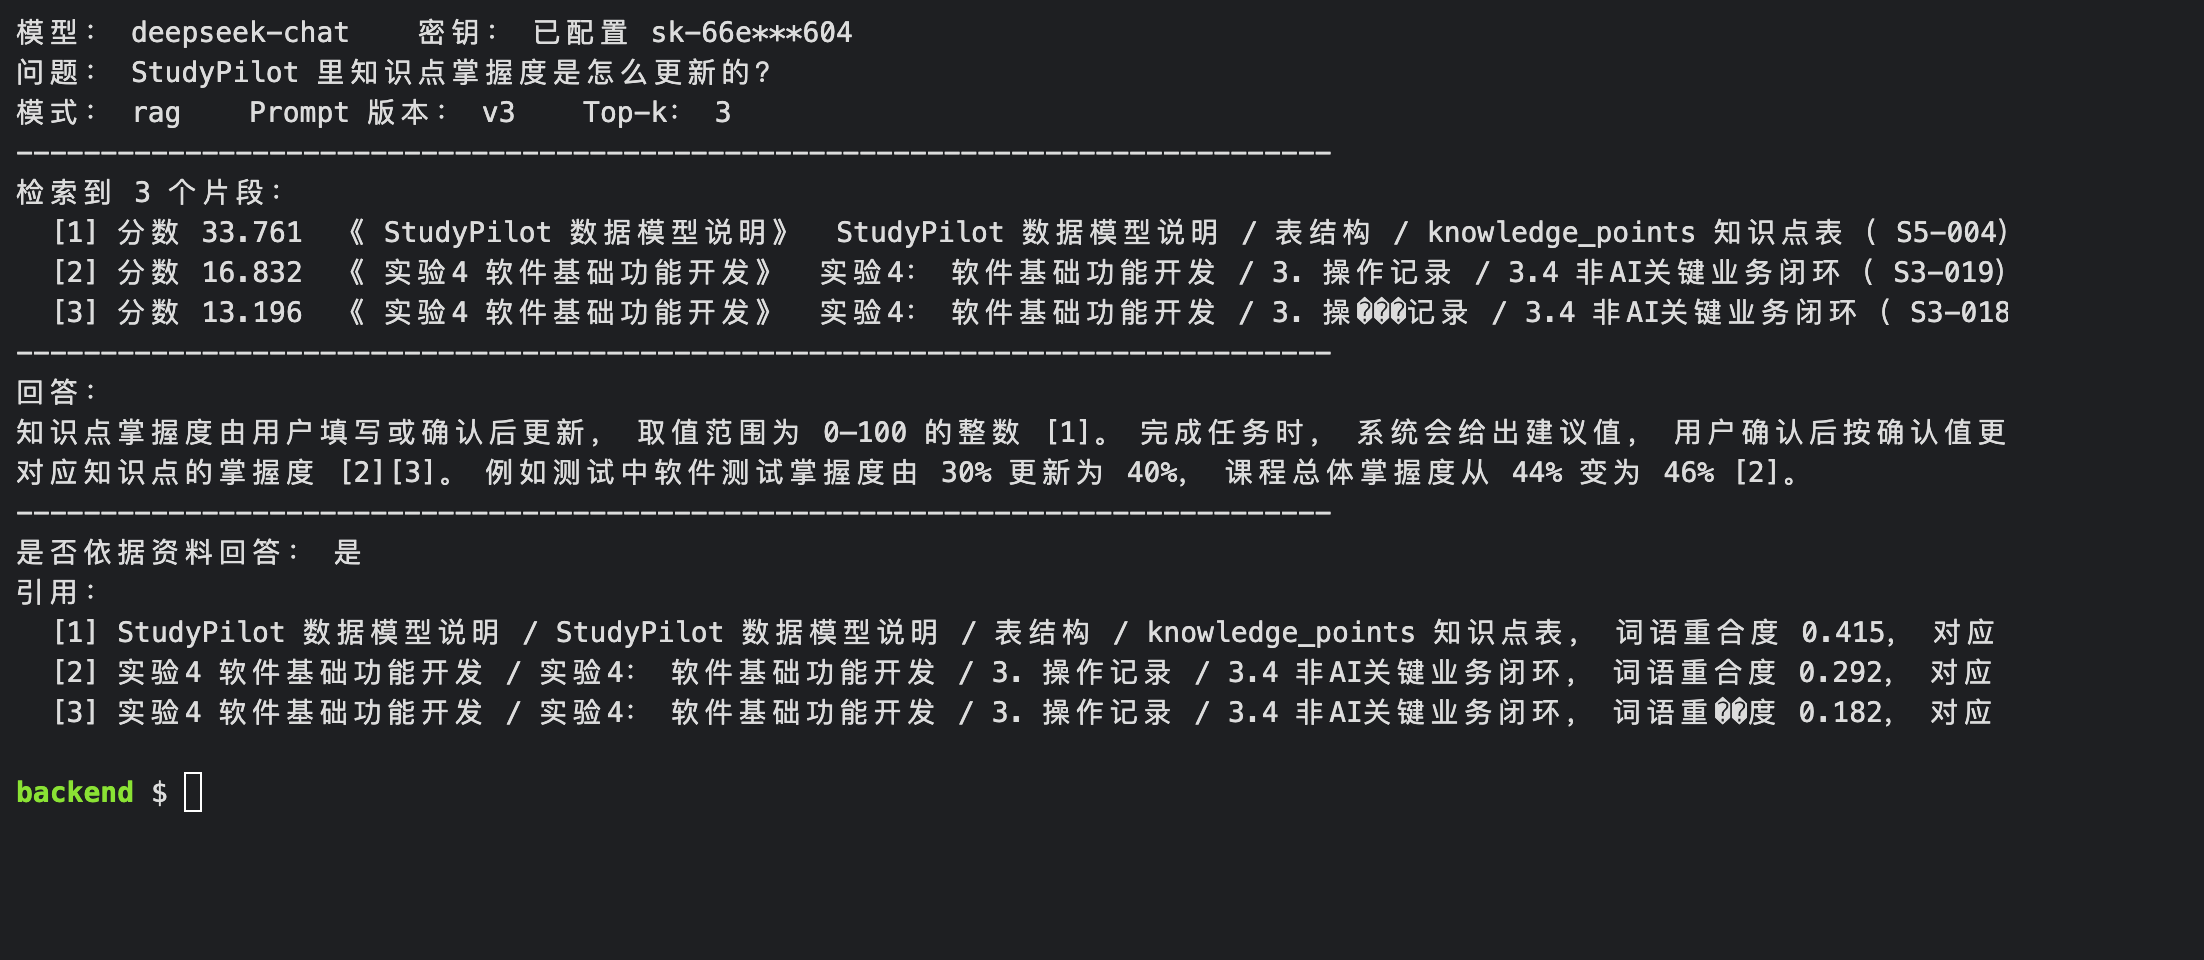
\includegraphics[width=0.96\textwidth]{e5-call-a.png}
\caption{一次完整调用：检索片段、回答与出处}
\end{figure}

\begin{figure}[H]
\centering
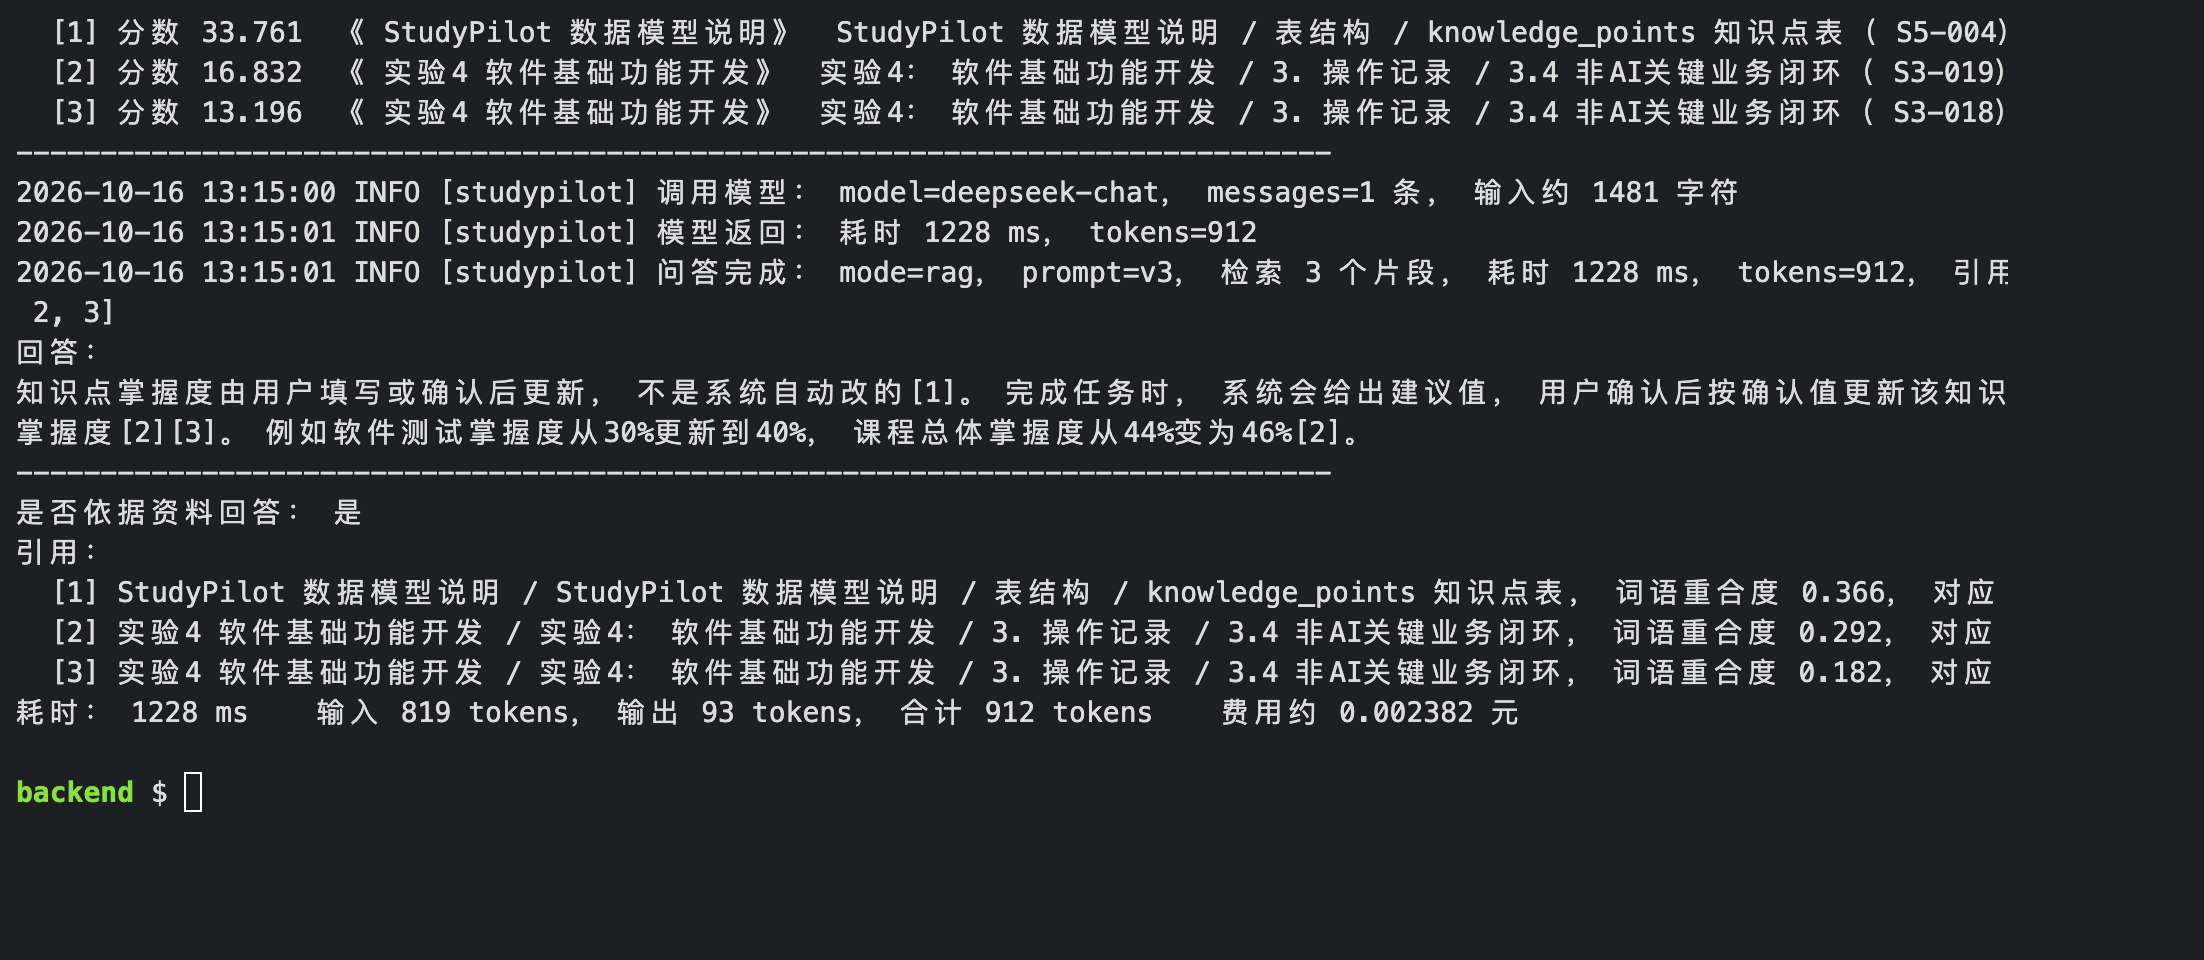
\includegraphics[width=0.96\textwidth]{e5-call.png}
\caption{调用返回：引用核对与Token、耗时、费用}
\end{figure}

调用失败处理按类型区分，接口返回统一结构的错误信息，程序不会中断。

\begin{table}[H]
\centering
\caption{三种调用失败情况的实测结果}
\footnotesize
\begin{tabularx}{\textwidth}{p{3.1cm}p{4.3cm}X p{1.6cm}}
\toprule
情况 & 错误码 & 提示信息 & 接口返回 \\
\midrule
API Key 无效 & LLM\_AUTH\_FAILED & 模型服务鉴权失败（401），请检查 API Key & HTTP 502 \\
响应超时（超时设为1毫秒） & LLM\_TIMEOUT & 模型服务响应超时（ConnectTimeout），请稍后重试 & HTTP 504 \\
服务地址不可达 & LLM\_CONNECTION\_ERROR & 无法连接模型服务，请检查网络或服务地址 & HTTP 503 \\
\bottomrule
\end{tabularx}
\end{table}

\begin{figure}[H]
\centering
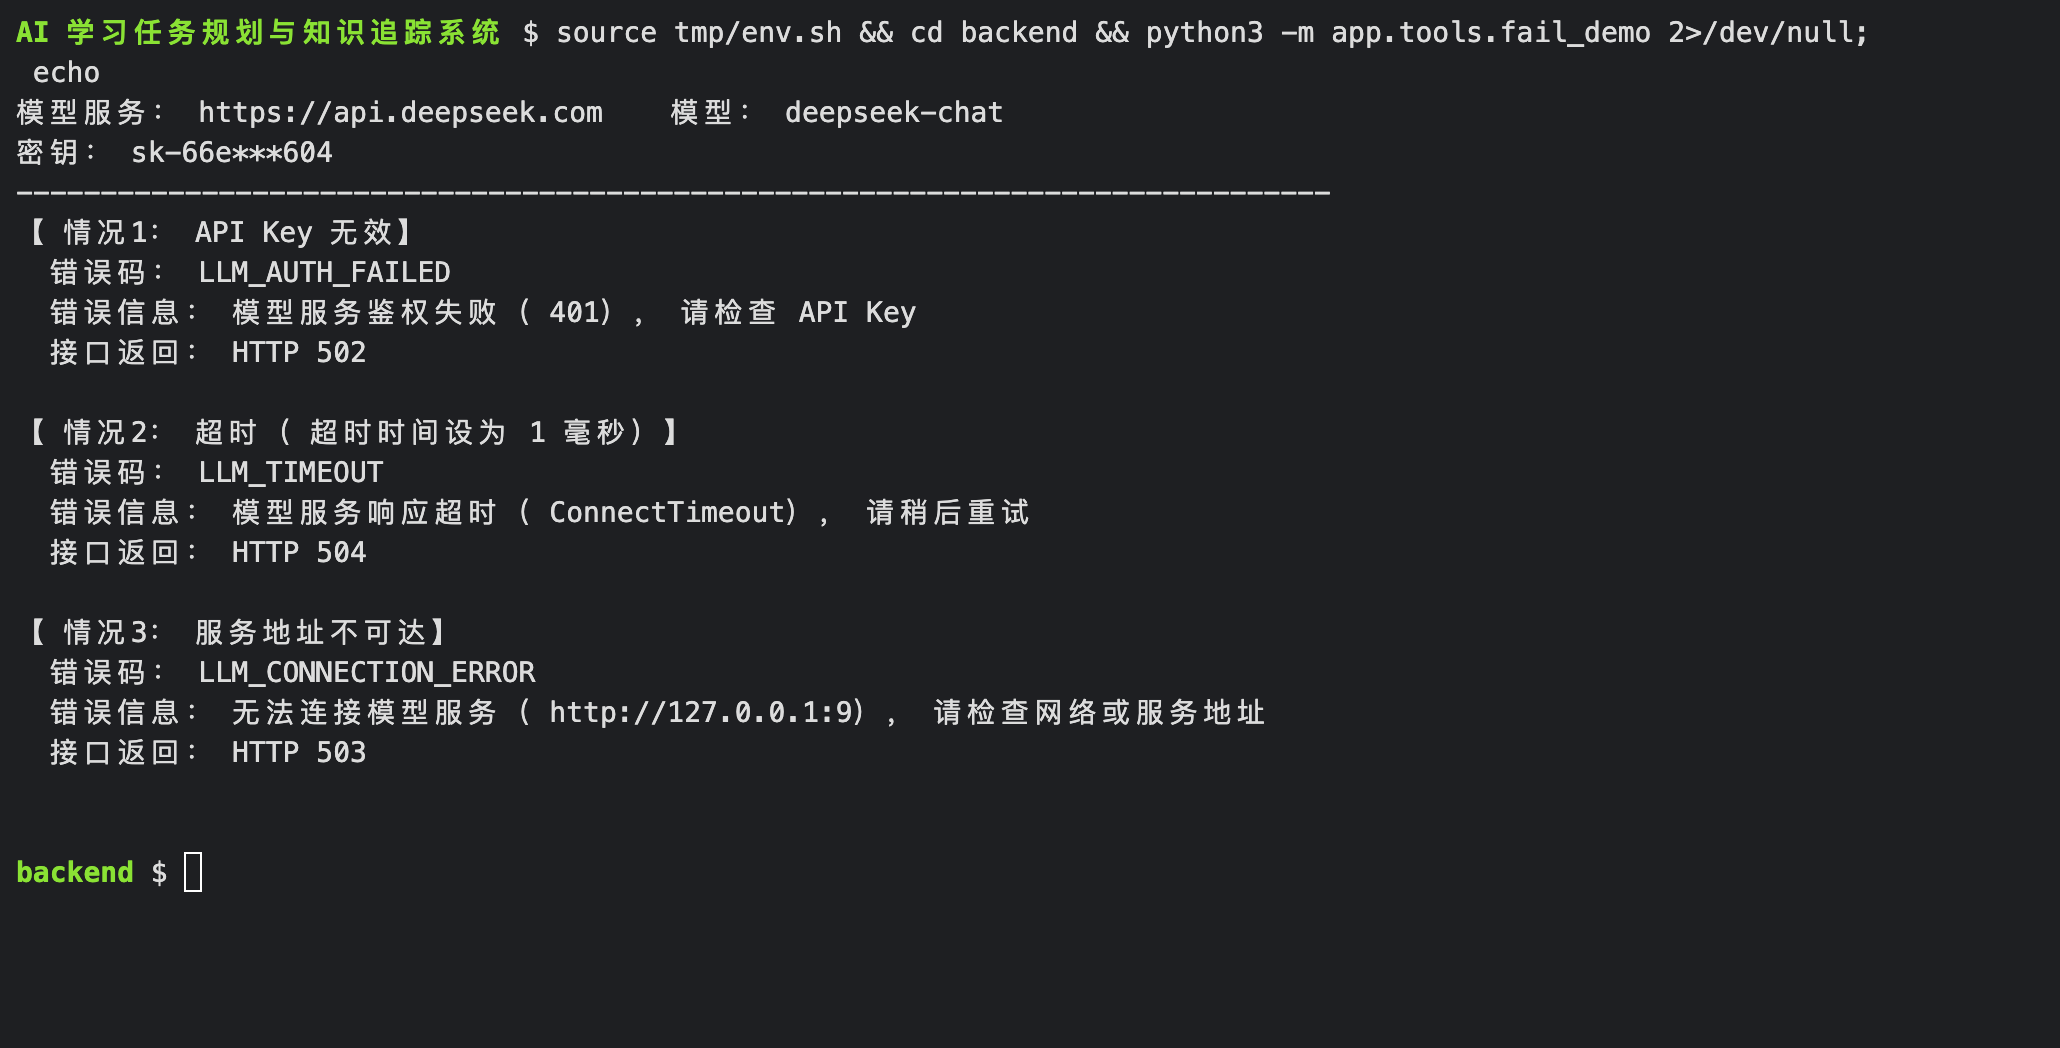
\includegraphics[width=0.9\textwidth]{e5-fail.png}
\caption{调用失败实测：鉴权失败、超时、地址不可达}
\end{figure}

结构化输出用“把自然语言学习要求解析成任务”来验证：字段为 title、minutes、date、point，日期用正则约束为 \texttt{YYYY-MM-DD}。正常输入一次通过；故意换成模型无法满足的结构（要求 priority、owner 字段）时，第一次校验失败，程序把校验错误回传给模型并要求只返回合法 JSON，第二次通过，整个过程耗时 1565 毫秒、386 tokens。

\begin{figure}[H]
\centering
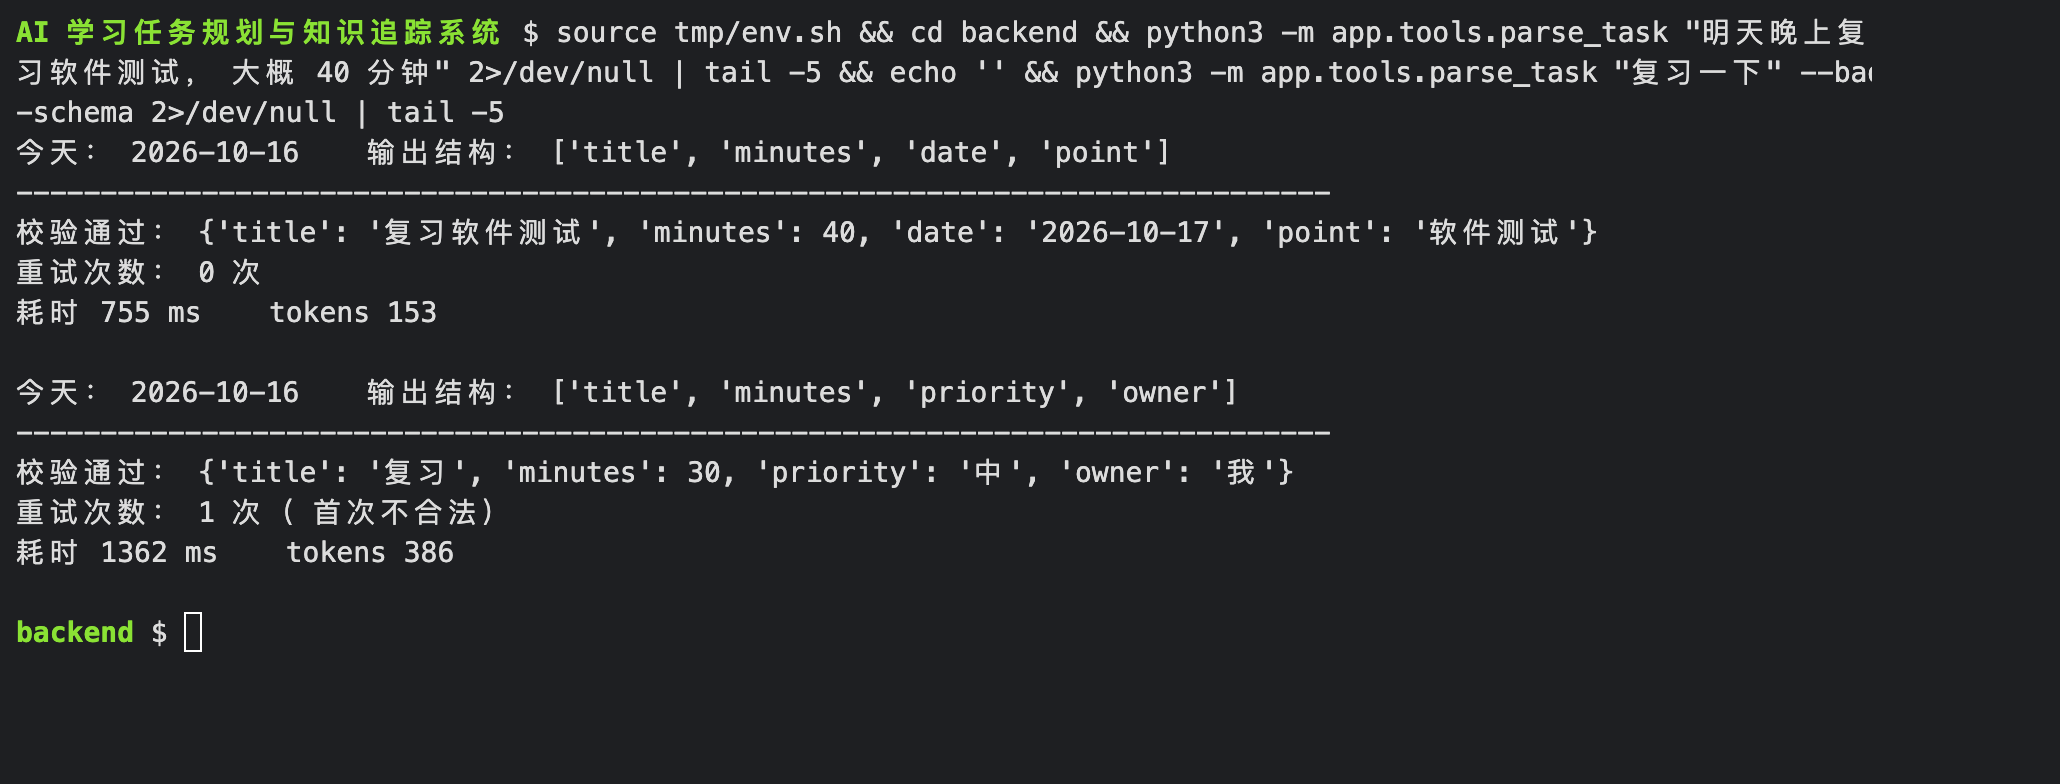
\includegraphics[width=0.9\textwidth]{e5-struct.png}
\caption{结构化输出：正常解析与校验失败后重试}
\end{figure}

三组输入的实测结果如下。第一组是正常问题，第二组缺少必要参数（第一版 Prompt 会直接讲设计内容，v3 修正后改为追问），第三组超出问答范围，检索没有达到阈值，直接返回资料不足，不调用模型。

\begin{table}[H]
\centering
\caption{三组输入的期望与实际结果}
\small
\begin{tabularx}{\textwidth}{p{1.6cm}p{4.3cm}X}
\toprule
类型 & 输入 & 实际结果 \\
\midrule
正常问题 & StudyPilot 里知识点掌握度是怎么更新的？ & 回答“由用户填写或确认后更新，不是系统自动改的”，并给出三处引用 \\
缺少必要信息 & 帮我设置考试目标 & 先说明无法直接设置，再列出需要补充的课程、考试日期、目标分数、每天可用时间 \\
超出任务范围 & 帮我写一首关于春天的诗 & 检索无结果，返回“资料不足：知识库中没有找到与该问题相关的内容”，未调用模型 \\
\bottomrule
\end{tabularx}
\end{table}

\begin{figure}[H]
\centering
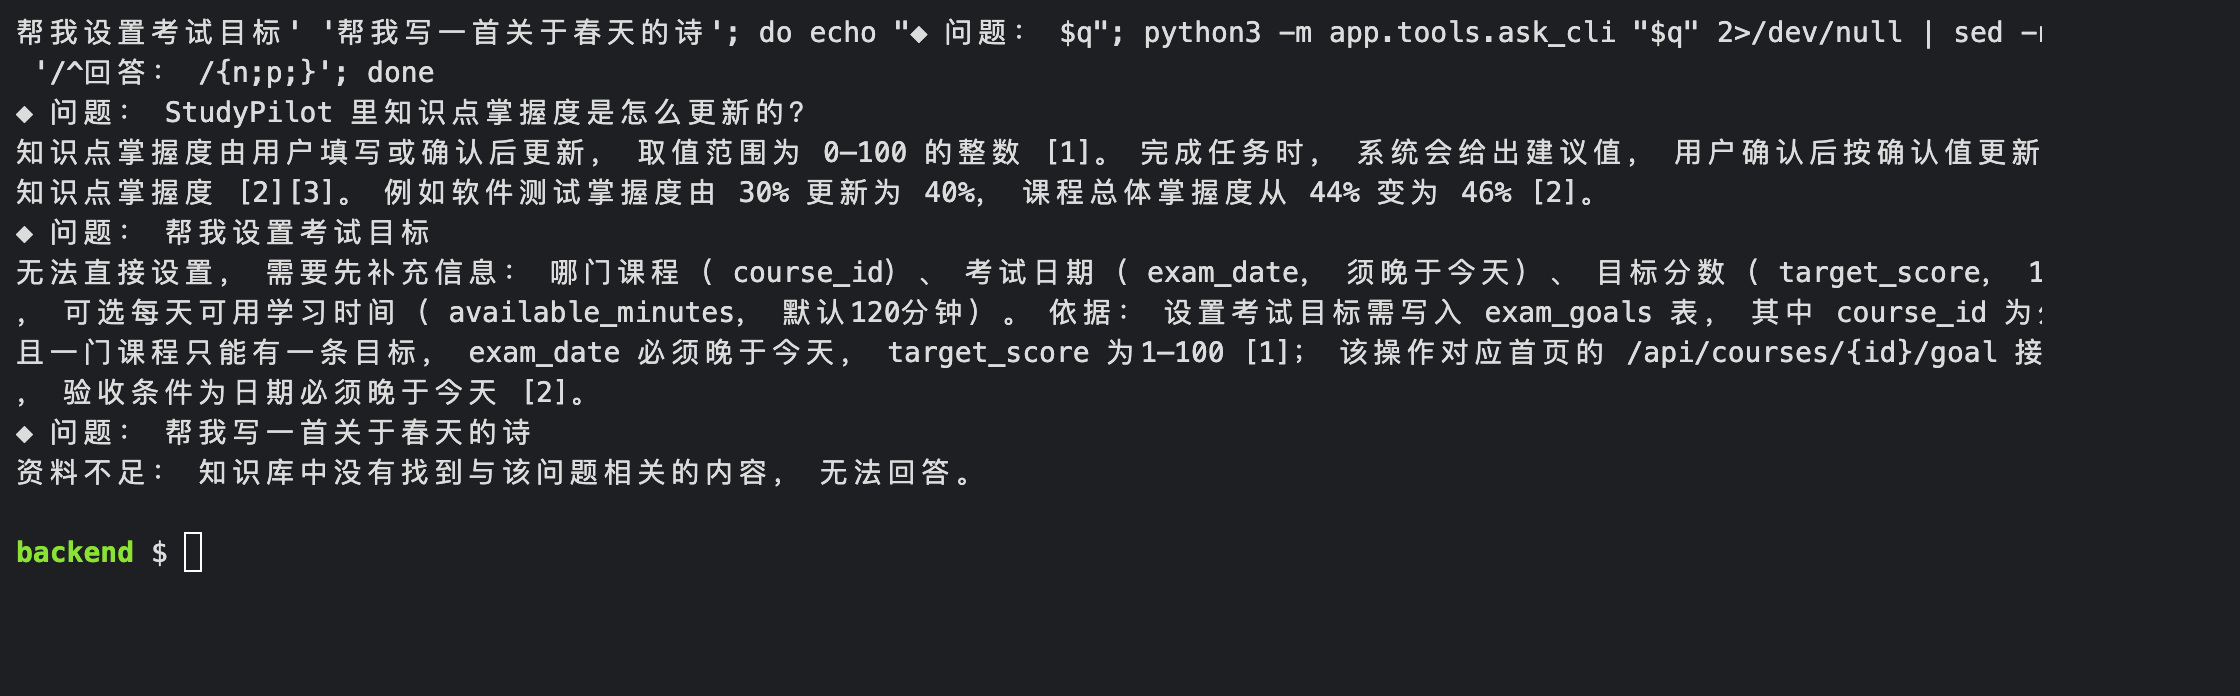
\includegraphics[width=0.96\textwidth]{e5-inputs.png}
\caption{三组输入的实际反馈}
\end{figure}

\subsection*{3.2 Prompt与上下文组织}

Prompt 模板放在 \texttt{backend/app/service/prompts.py}，任务要求与用户问题分开：模板里写清回答范围、长度、引用格式、信息不足和超范围时的处理，最后才是资料和用户问题。版本变化见表5-4，实际发送给模型的完整输入见图5-6和图5-7。

\begin{table}[H]
\centering
\caption{Prompt修改记录}
\small
\begin{tabularx}{\textwidth}{p{1.1cm}p{3.0cm}X p{3.6cm}}
\toprule
版本 & 原版本问题 & 修改内容 & 结果变化 \\
\midrule
v1 & RAG 只写“请根据资料回答问题” & 无格式要求，模型自由发挥 & 回答偏长、用 Markdown 罗列，没有编号引用，出处无法核对 \\
v2 & 回答长度和引用不规范 & 增加只依据资料、250字以内、句末标注 [1]、资料不足时置 sufficient=false、只输出 JSON & 回答变短，引用可直接核对到片段；无答案时明确说资料不足 \\
v3 & 缺少参数的操作请求（如“帮我设置考试目标”）被当成普通问题回答 & 增加一条：操作请求缺少参数时先列出需要补充的信息 & 同一问题改为追问课程、考试日期、目标分数、每天可用时间 \\
\bottomrule
\end{tabularx}
\end{table}

\begin{figure}[H]
\centering
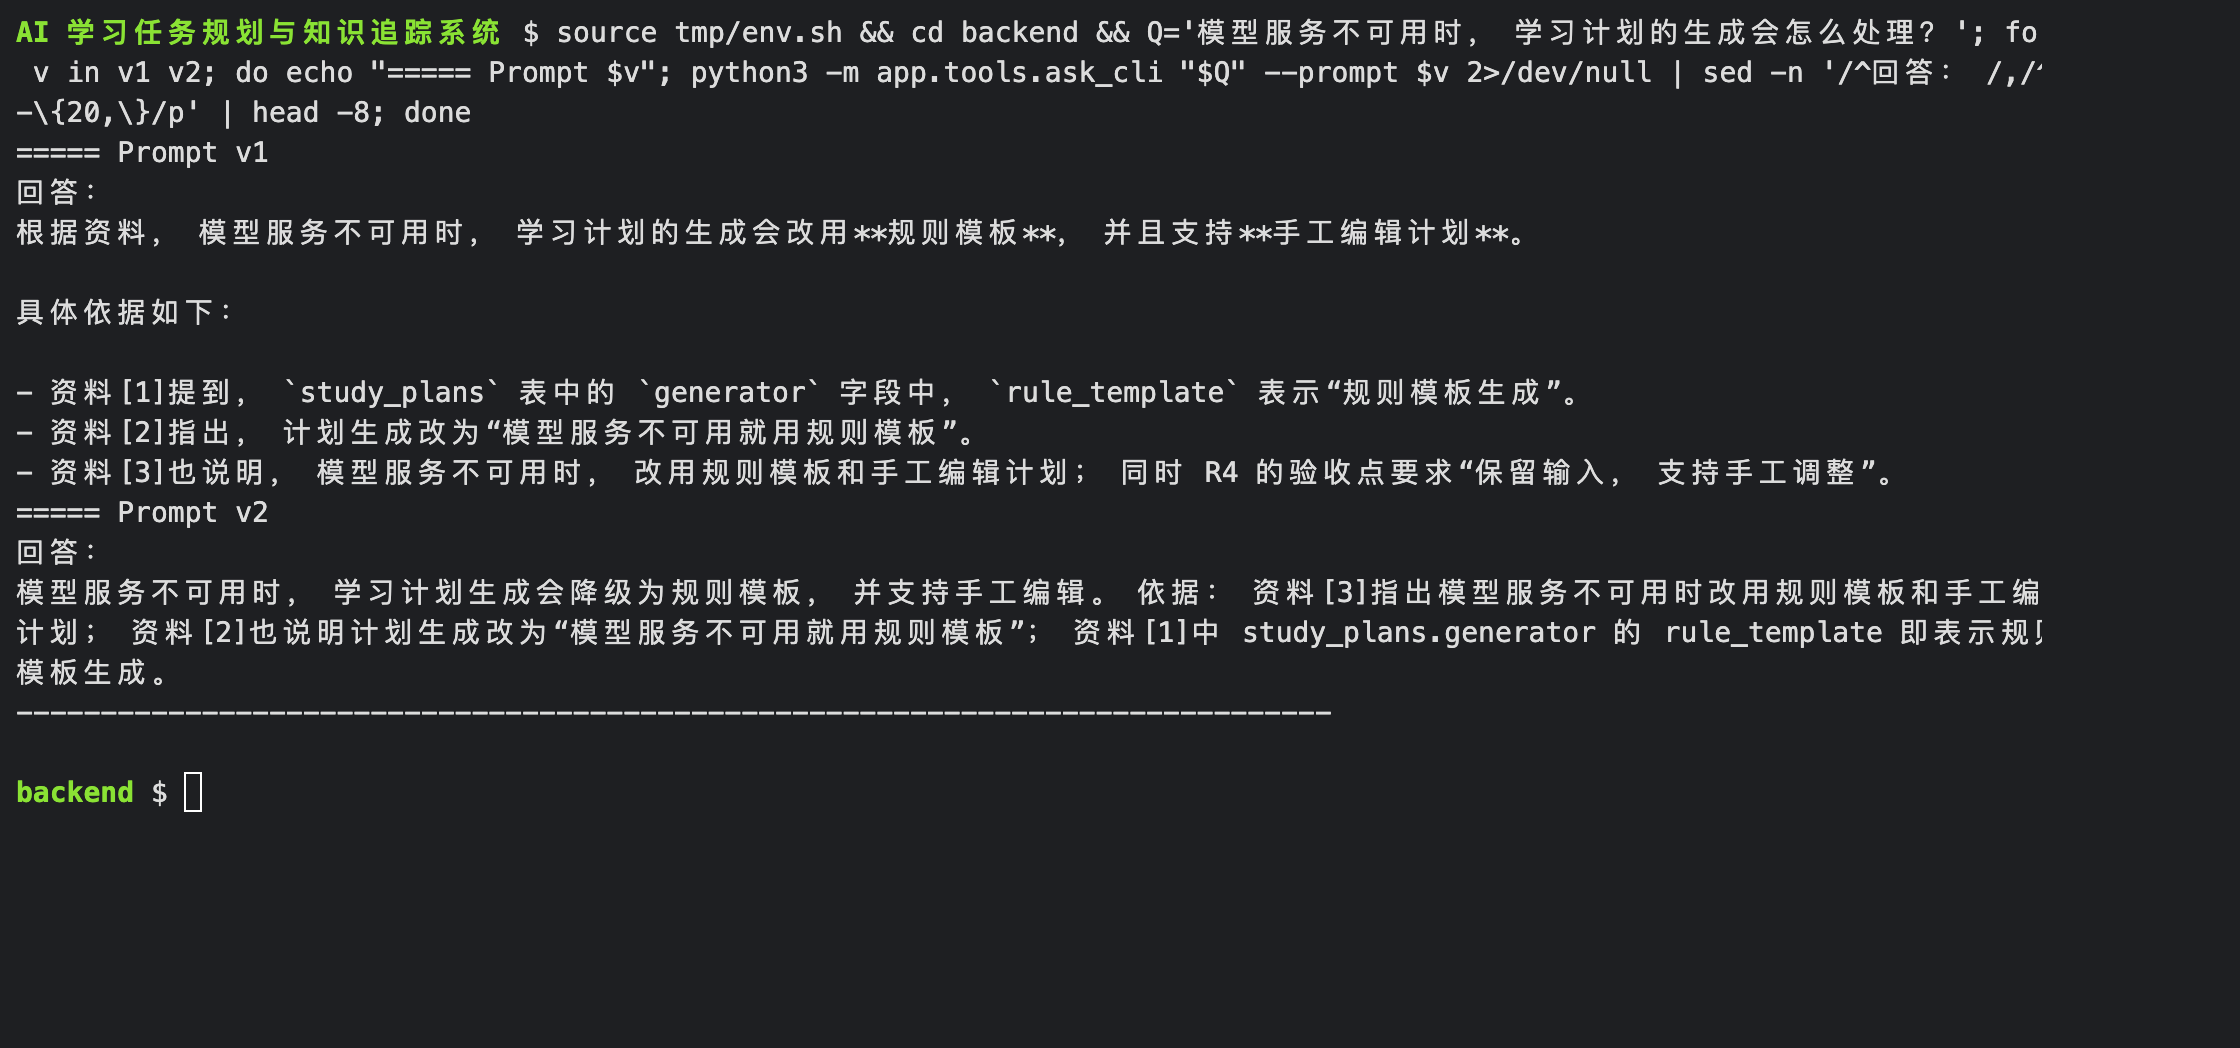
\includegraphics[width=0.9\textwidth]{e5-prompt.png}
\caption{Prompt v1（上）与 v2（下）对同一问题的回答对比}
\end{figure}

\begin{figure}[H]
\centering
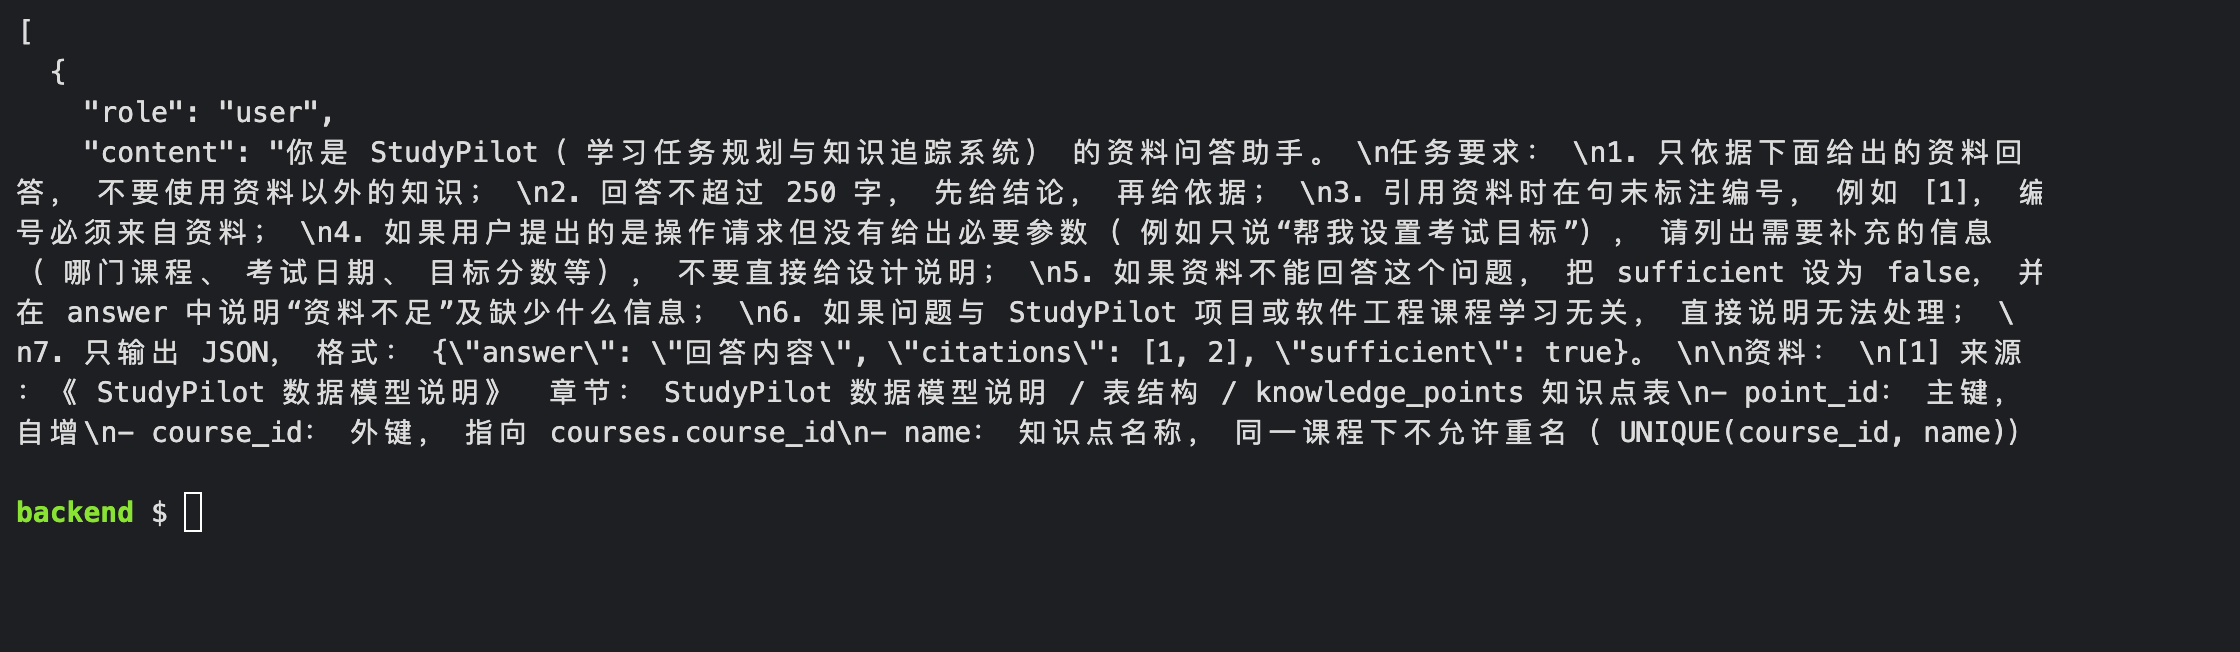
\includegraphics[width=0.96\textwidth]{e5-messages-head.png}
\caption{实际发送给模型的输入：任务要求与资料编号}
\end{figure}

\begin{figure}[H]
\centering
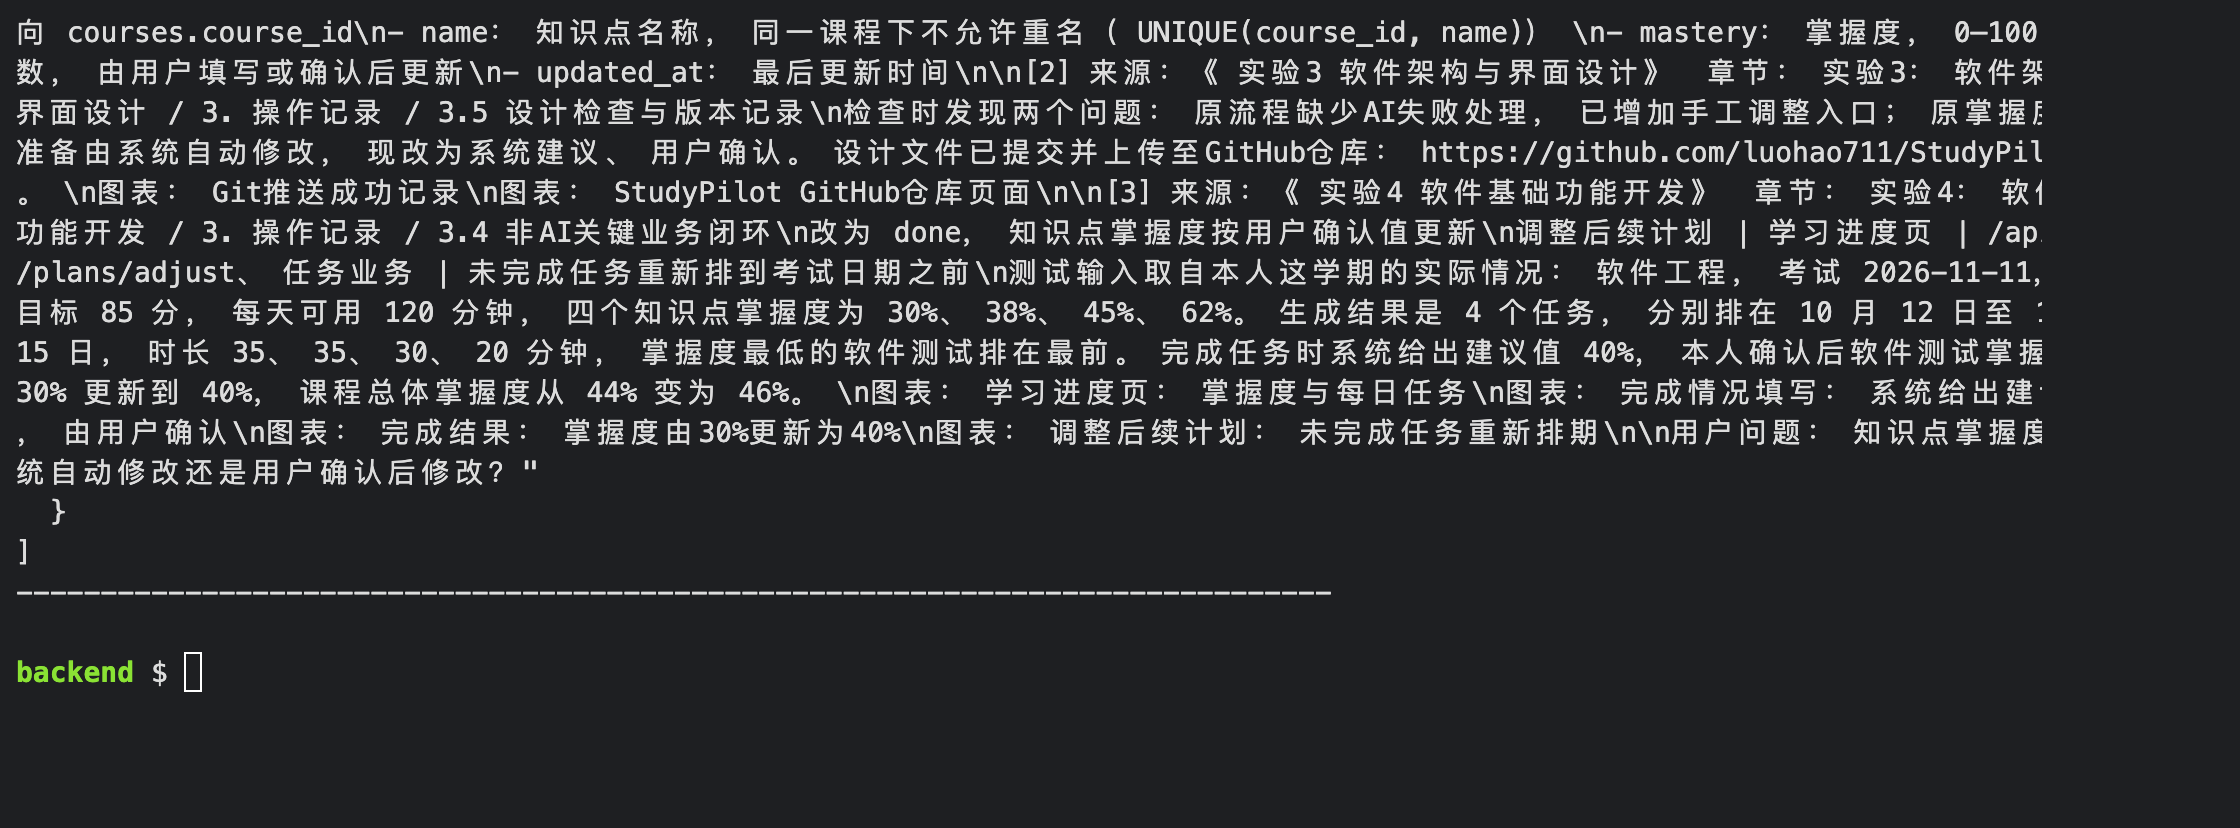
\includegraphics[width=0.96\textwidth]{e5-messages.png}
\caption{实际输入中的资料内容与用户问题}
\end{figure}

上下文检查发现两类问题：一是检索排在后面的片段与问题无关（例如问架构却带回 LaTeX 编译命令），二是相邻片段有 80 字重叠，同一句话可能在上下文里出现两次（本次样例重复 25 字）。按“分数不低于最高分 60\%”精简后，上下文从 955 字降到 604 字（减少 37\%），prompt tokens 从 805 降到 612，回答和引用都没有变化。

\begin{figure}[H]
\centering
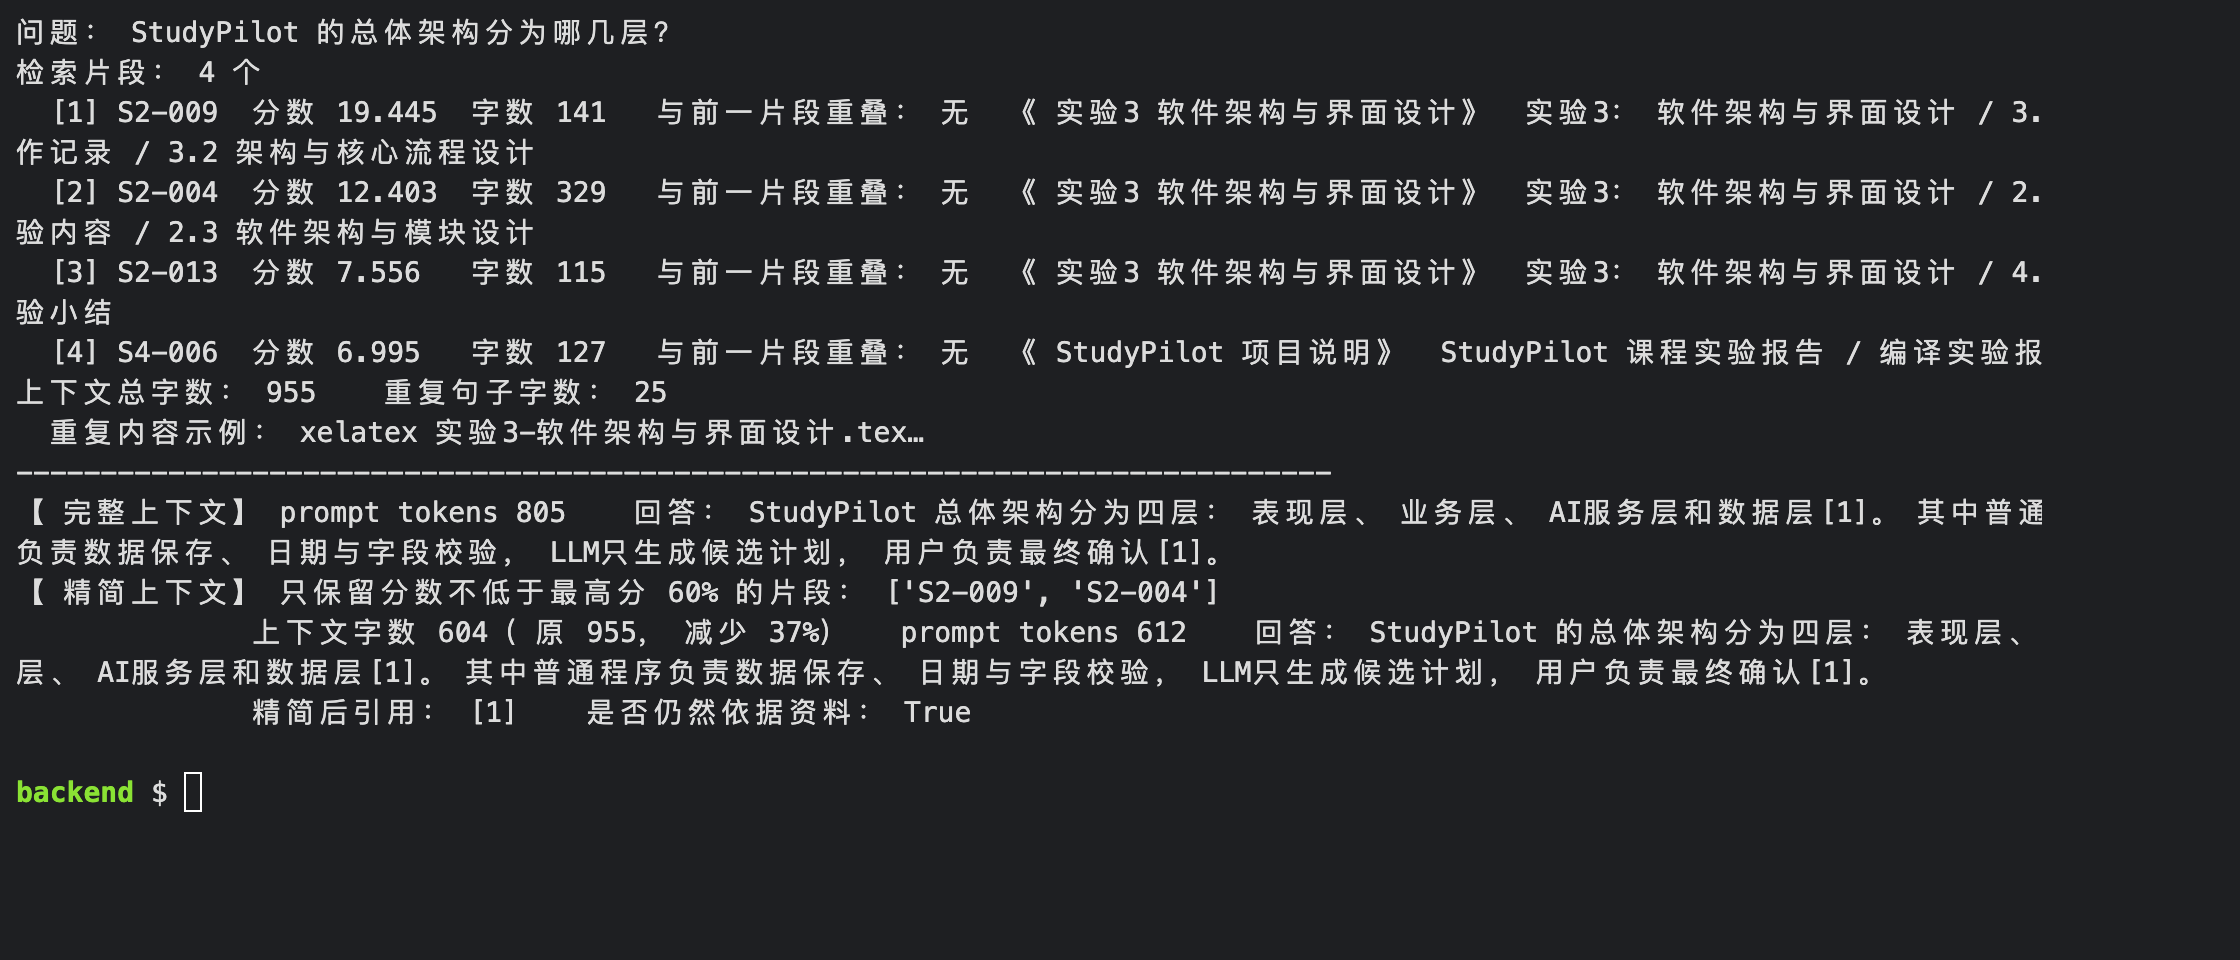
\includegraphics[width=0.96\textwidth]{e5-context.png}
\caption{上下文检查：无关片段、重复内容与精简前后对比}
\end{figure}

\subsection*{3.3 知识库与切分策略}

知识库共 5 篇资料，全部是本人编写的项目文档，来源明确、可以公开，不包含他人隐私和密钥。资料清单放在 \texttt{backend/kb/sources.json}，每条记录使用权限和隐私处理方式。

\begin{table}[H]
\centering
\caption{知识库资料清单}
\small
\begin{tabularx}{\textwidth}{p{1.0cm}p{4.4cm}p{5.4cm}p{1.6cm}p{1.4cm}}
\toprule
编号 & 资料 & 来源文件 & 字数 & 片段数 \\
\midrule
S1 & 实验2 个人软件选题与需求分析 & reports/experiment2/…tex & 3957 & 17 \\
S2 & 实验3 软件架构与界面设计 & reports/experiment3/…tex & 3025 & 13 \\
S3 & 实验4 软件基础功能开发 & reports/experiment4/…tex & 7179 & 29 \\
S4 & StudyPilot 项目说明 & README.md & 991 & 7 \\
S5 & StudyPilot 数据模型说明 & backend/kb/source/数据模型说明.md & 1696 & 8 \\
\bottomrule
\end{tabularx}
\end{table}

清理与切分：LaTeX 报告先转成纯文本，去掉导言区、命令和图片，表格按行转成“单元格 | 单元格”，图只有标题时保留“图表：标题”一行；然后按标题切成小节，小节内按段落合并到 420 字左右，同一小节被切开时保留上一片段末尾 80 字作为重叠。更新方法是修改源文件后重新执行 \texttt{python3 -m app.tools.build\_kb}，片段编号会重新生成。

\begin{figure}[H]
\centering
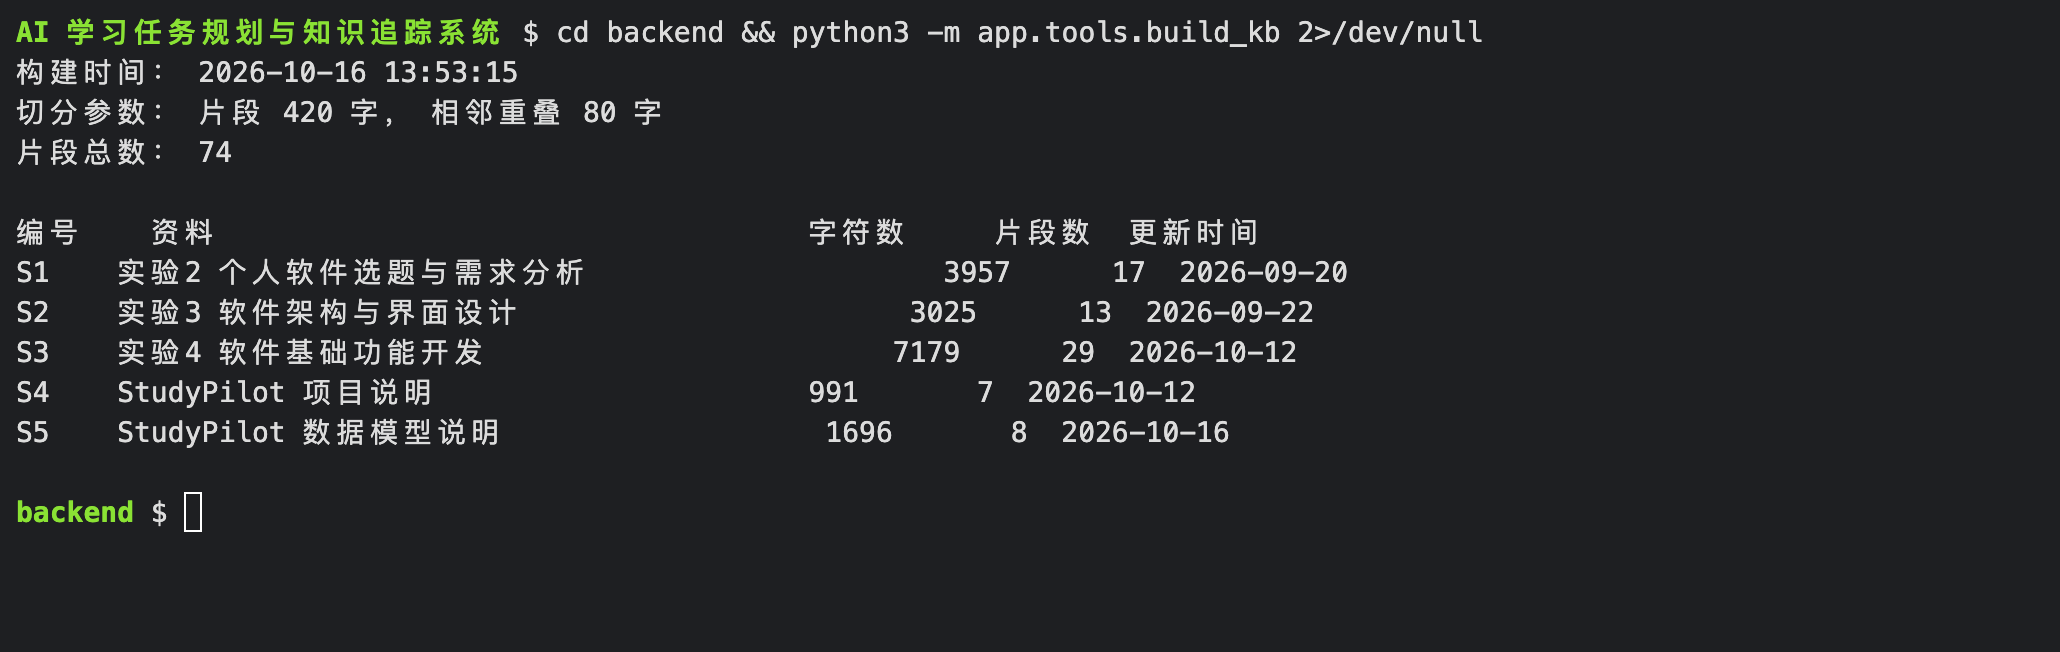
\includegraphics[width=0.96\textwidth]{e5-kb.png}
\caption{知识库构建结果：5篇资料、74个片段}
\end{figure}

抽查了 3 个片段：S2-009（架构分层，141 字，无重叠）、S5-004（知识点表字段，157 字，无重叠）、S3-019（掌握度更新与验收，有重叠）。检查结果：关键句子完整，“系统分为表现层、业务层、AI服务层和数据层”没有在切分处断开；来源路径、章节和更新时间都能对应回原资料；带重叠的片段开头确实重复了上一片段的结尾，用于避免跨片段的问题漏检。

\begin{figure}[H]
\centering
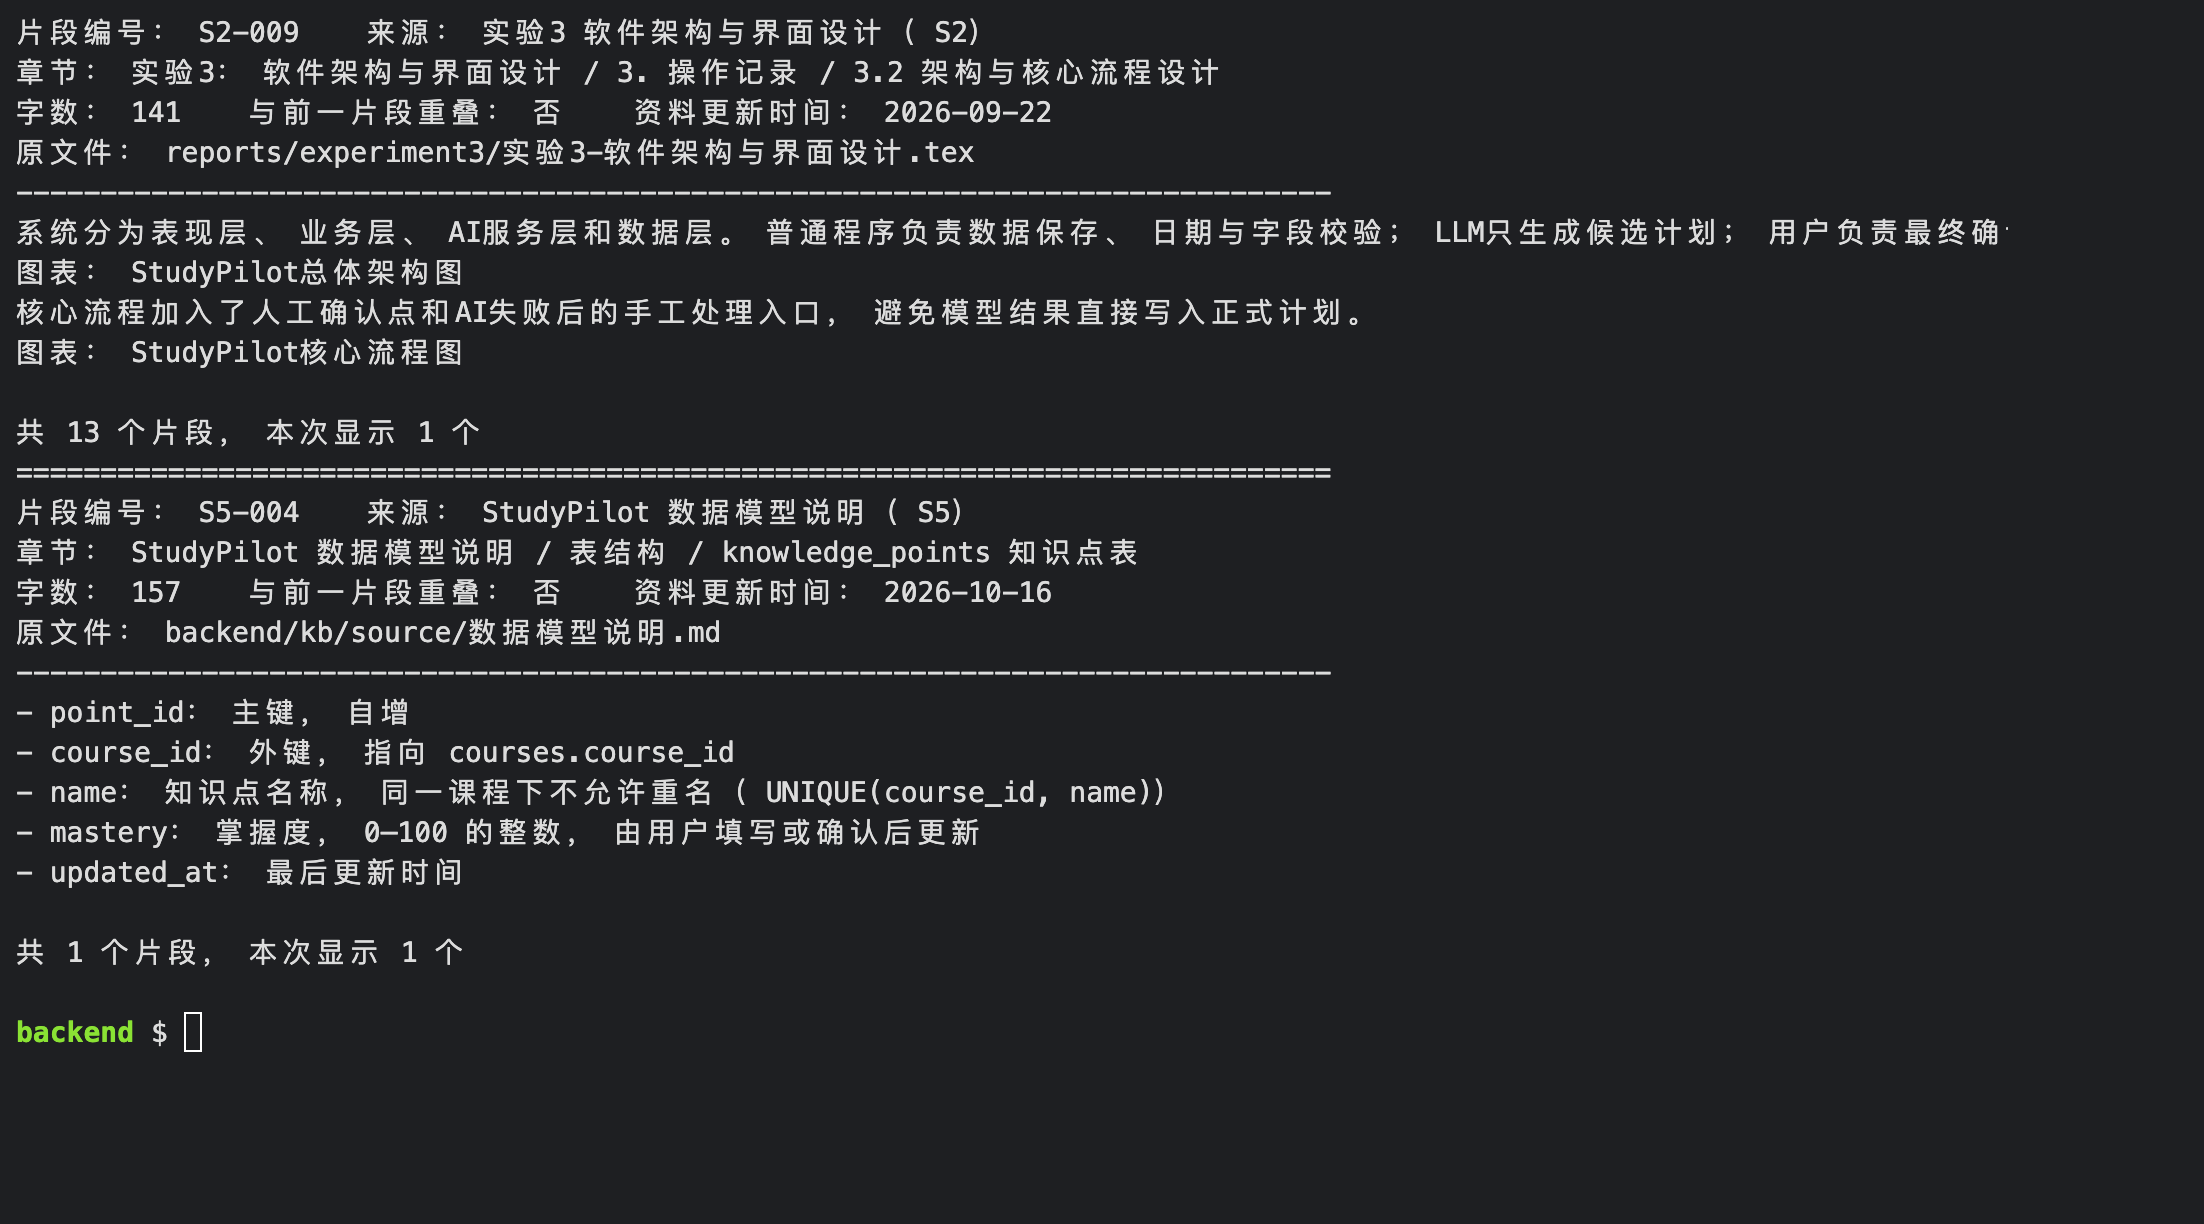
\includegraphics[width=0.96\textwidth]{e5-chunks.png}
\caption{片段抽查一：S2-009与S5-004的内容与元数据}
\end{figure}

\begin{figure}[H]
\centering
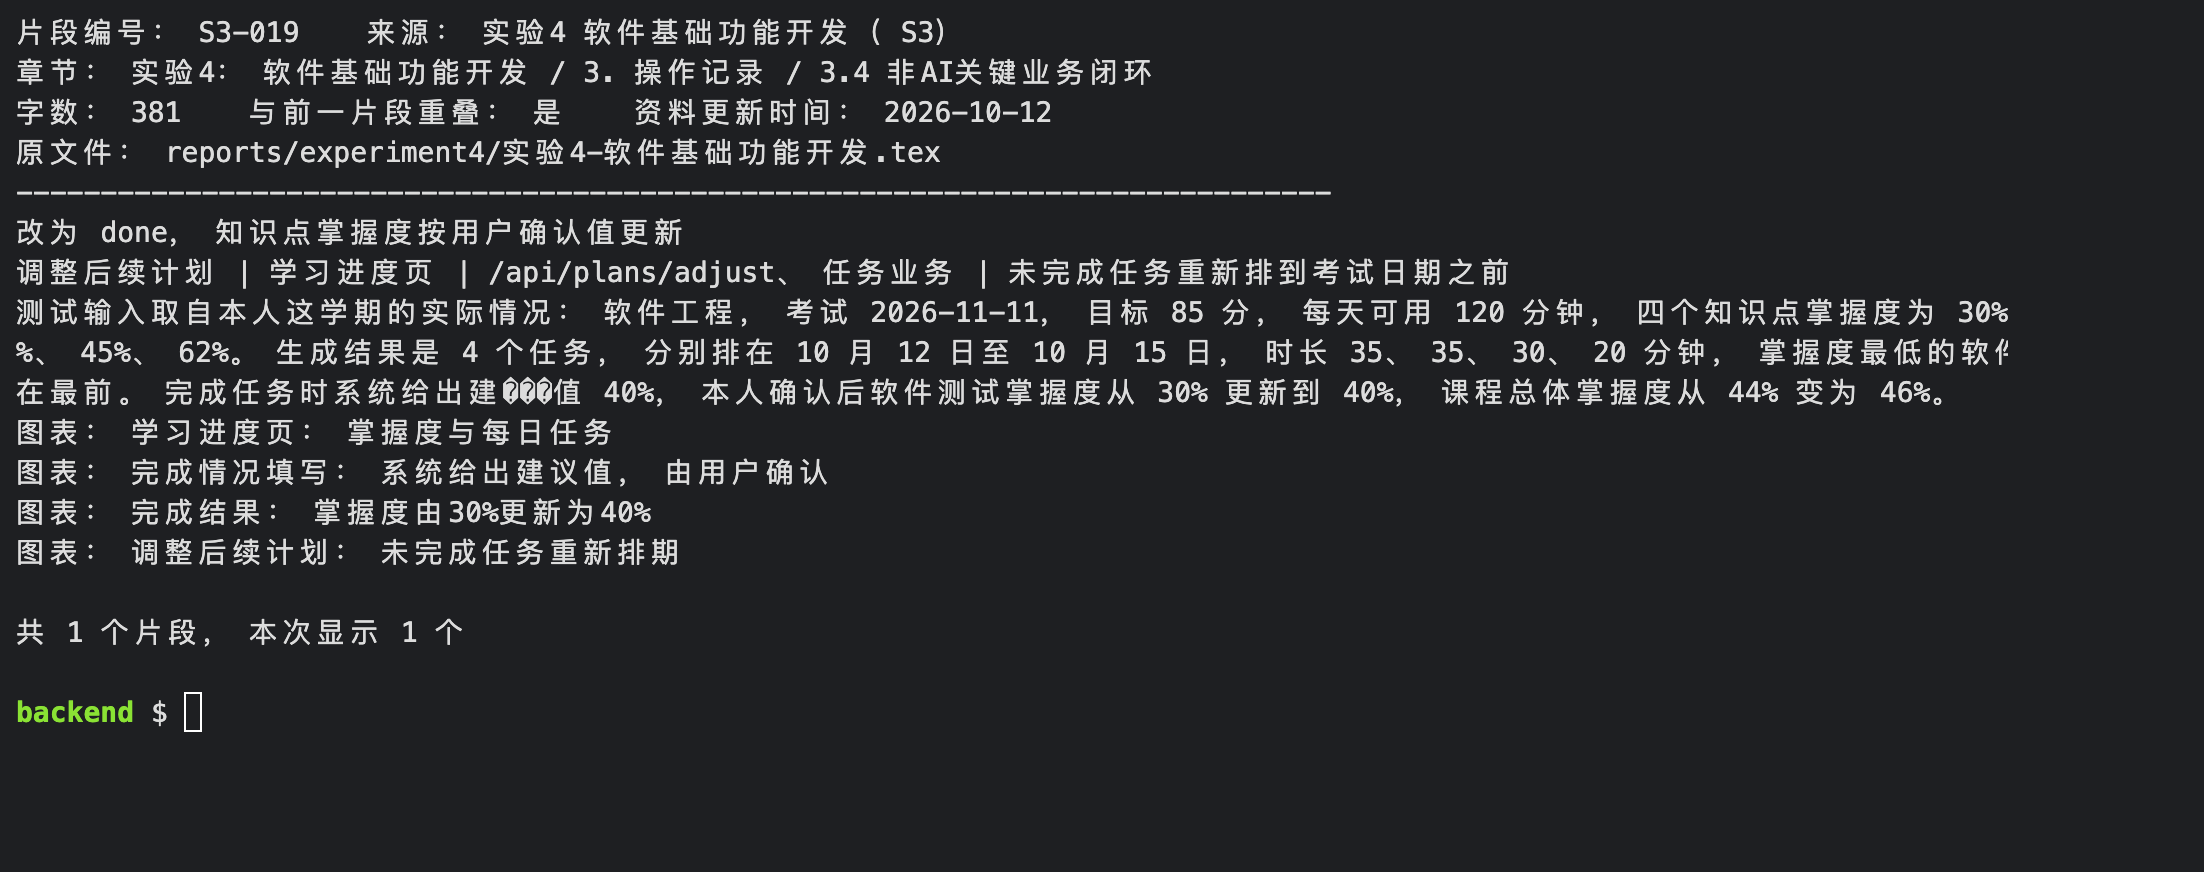
\includegraphics[width=0.96\textwidth]{e5-chunks2.png}
\caption{片段抽查二：S3-019的内容与重叠标记}
\end{figure}

\subsection*{3.4 检索与RAG最小链路}

检索用关键词方法：中文按二字切分、英文按单词切分，用 BM25 排序（k1=1.5，b=0.75），并加入标题字段加权和同义词扩展。选择理由是没有配置嵌入模型，资料量只有几十个片段，关键词检索的排序依据可以逐项核对，不需要额外的模型服务。主要参数见表5-6。

\begin{table}[H]
\centering
\caption{切分与检索参数}
\small
\begin{tabularx}{\textwidth}{p{3.4cm}X}
\toprule
项目 & 取值与说明 \\
\midrule
片段大小 & 420 字，相邻片段重叠 80 字 \\
分词方式 & 中文二字组合 + 英文单词，去停用词 \\
排序方法 & BM25，标题字段权重 1.2 \\
同义词扩展 & 权重 0.6，例如“数据库→表/字段/主键/外键” \\
相关性阈值 & 10 分，低于阈值视为没有相关资料 \\
Top-k & 默认 3，页面可调 1—8 \\
\bottomrule
\end{tabularx}
\end{table}

阈值是抽查后定的：有答案的问题最高分在 15.9—33.2 之间，与项目无关的问题在 6.9 分以下，取 10 分可以分开这两类；话题相关但资料没有答案的问题落在中间，交给模型判断并把 sufficient 置为 false。

\begin{figure}[H]
\centering
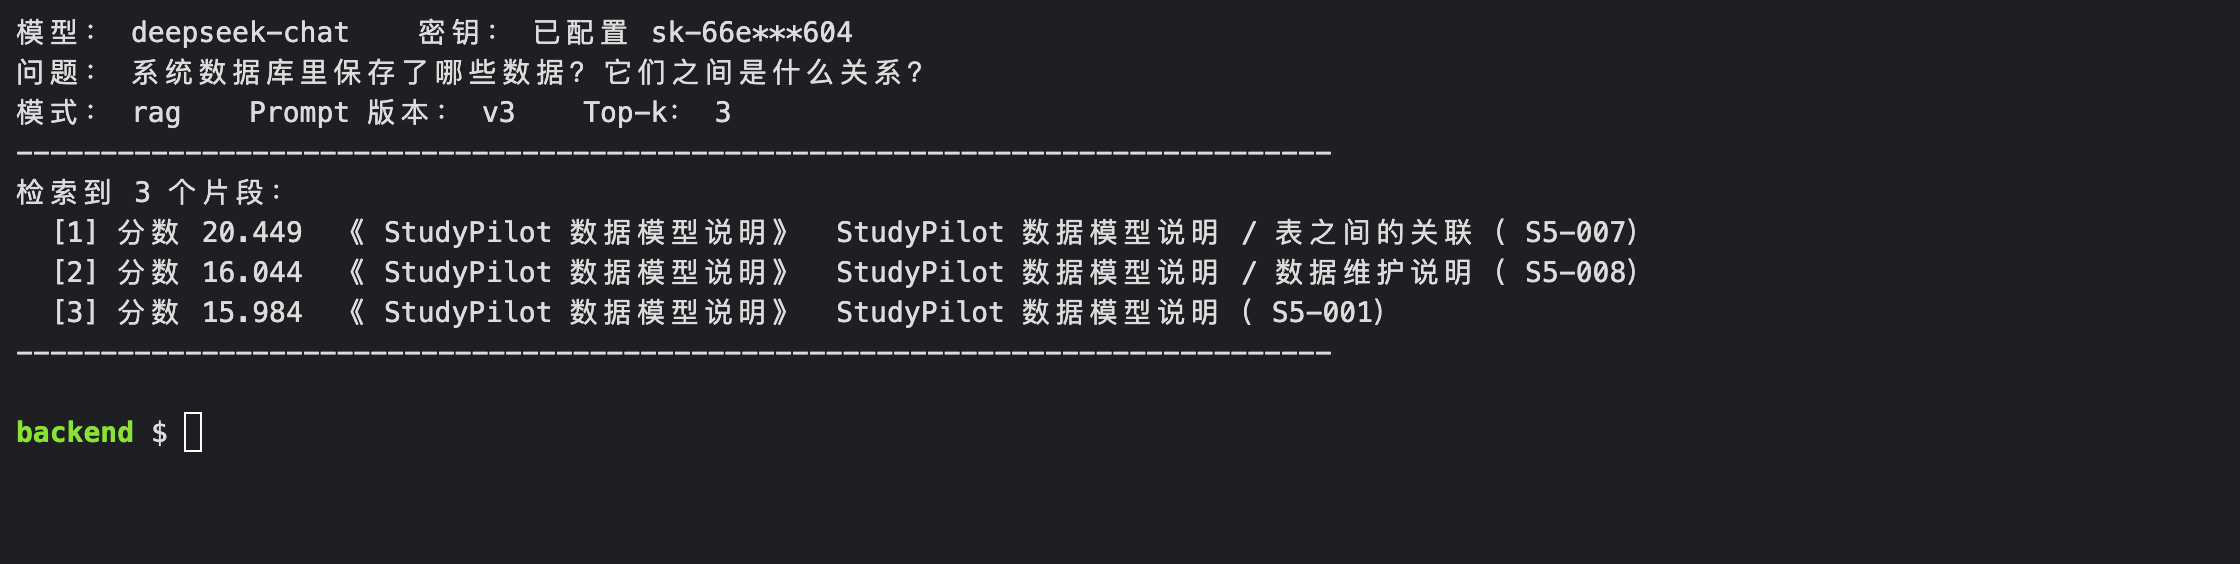
\includegraphics[width=0.96\textwidth]{e5-retrieval.png}
\caption{一次查询的Top-3片段与BM25分数}
\end{figure}

样例检查发现过一次检索失败：问“系统数据库里保存了哪些数据？它们之间是什么关系？”时，前 3 个片段都是实验3的设计说明，没有检索到数据模型的内容，回答只能给出资料不足。原因是问题和资料用词不一致（问“数据库、数据”，资料里写的是“表、字段、主键”），而且正文里的通用词太多。加入标题加权和同义词扩展后，数据模型说明的“表之间的关联”片段排到第 1，回答也正确了。

\begin{table}[H]
\centering
\caption{检索改进前后对比（同一个问题）}
\small
\begin{tabularx}{\textwidth}{p{2.6cm}X p{3.4cm}}
\toprule
阶段 & Top-3 片段（分数） & 回答情况 \\
\midrule
改进前 & S2-004(11.2)、S2-001(7.4)、S2-006(6.1) & 资料不足，未回答 \\
改进后 & S5-007(20.4)、S5-008(16.0)、S5-001(16.0) & 正确列出用户、课程、考试目标、知识点、计划、任务及关联，并给出引用 \\
\bottomrule
\end{tabularx}
\end{table}

回答生成后做引用核对：检查编号是否在检索结果范围内，并计算被引用片段与回答的词语重合度，低于 0.12 标记为需要人工复核，编号越界直接判为不可靠。本轮对比测试中 RAG 组共引用 12 处，逐条检查全部对应。

资料不足分两种处理：检索完全没有结果时（如“项目开发一共花了多少钱”）直接返回资料不足，不调用模型；检索到了片段但资料回答不了时（如“用的是哪种知识追踪算法”），把 sufficient 置为 false，并在回答里说明缺少什么信息。

\begin{figure}[H]
\centering
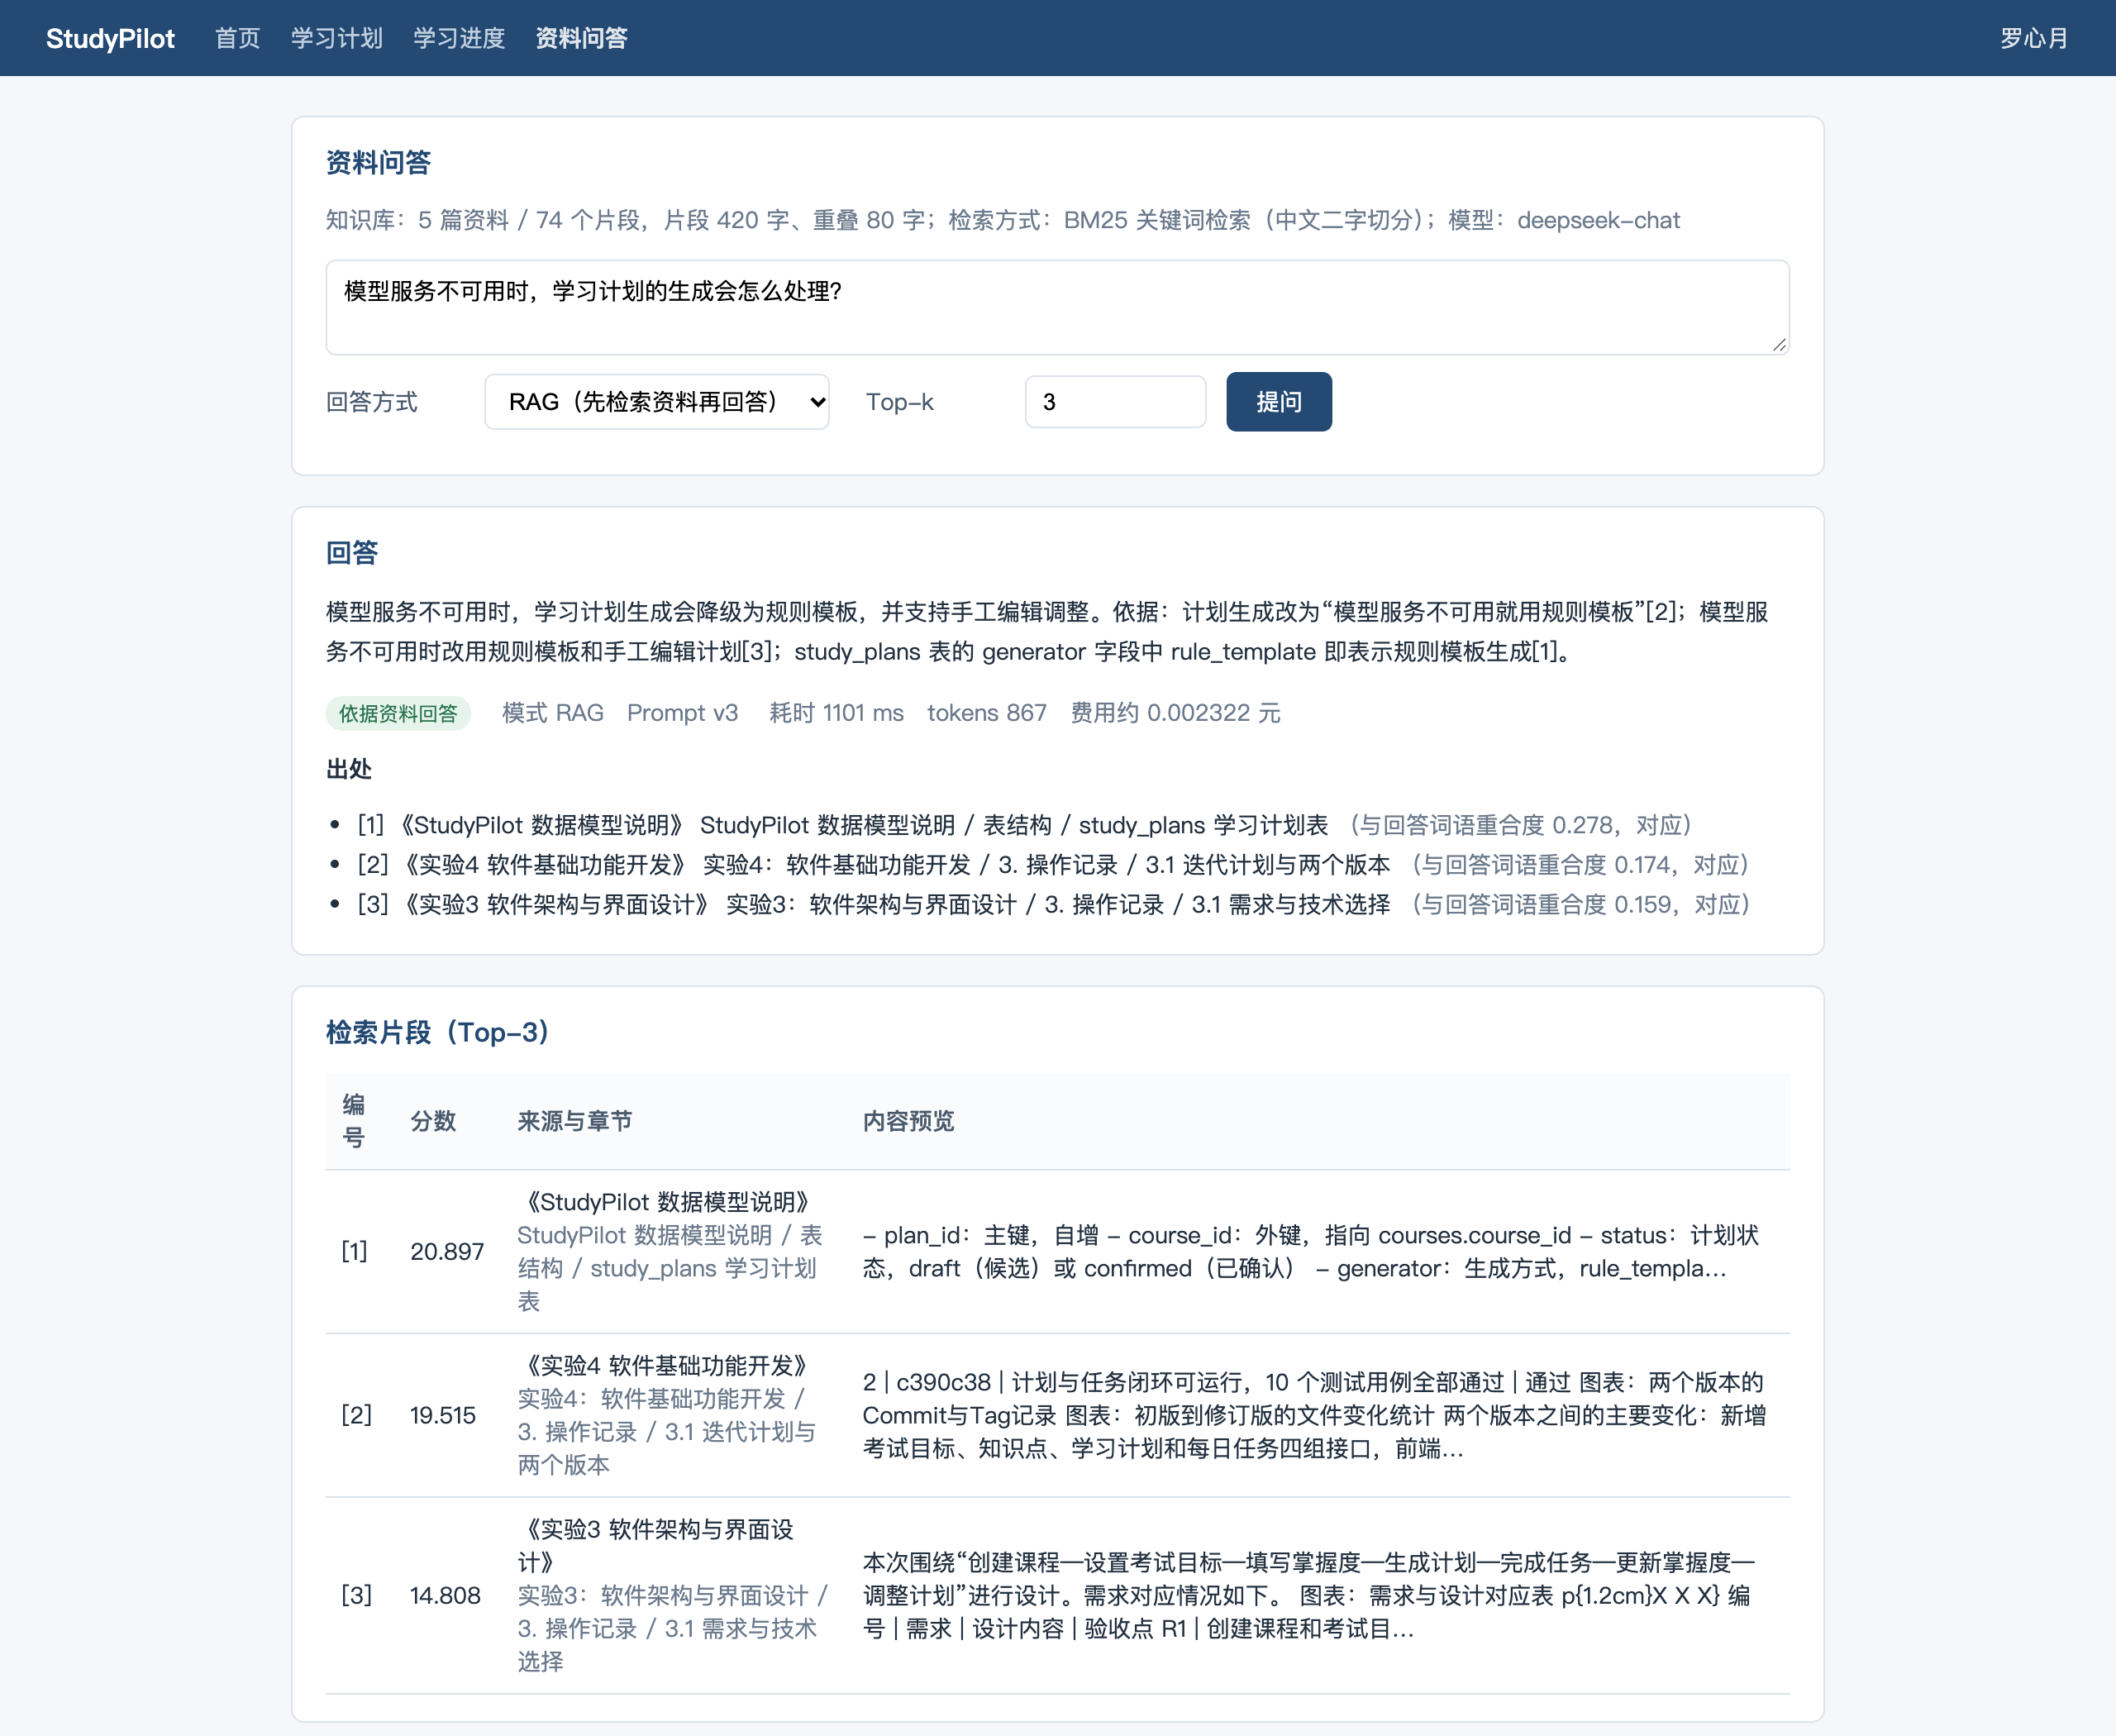
\includegraphics[width=0.88\textwidth]{e5-ask-rag.png}
\caption{页面入口：RAG回答、出处与检索片段}
\end{figure}

\begin{figure}[H]
\centering
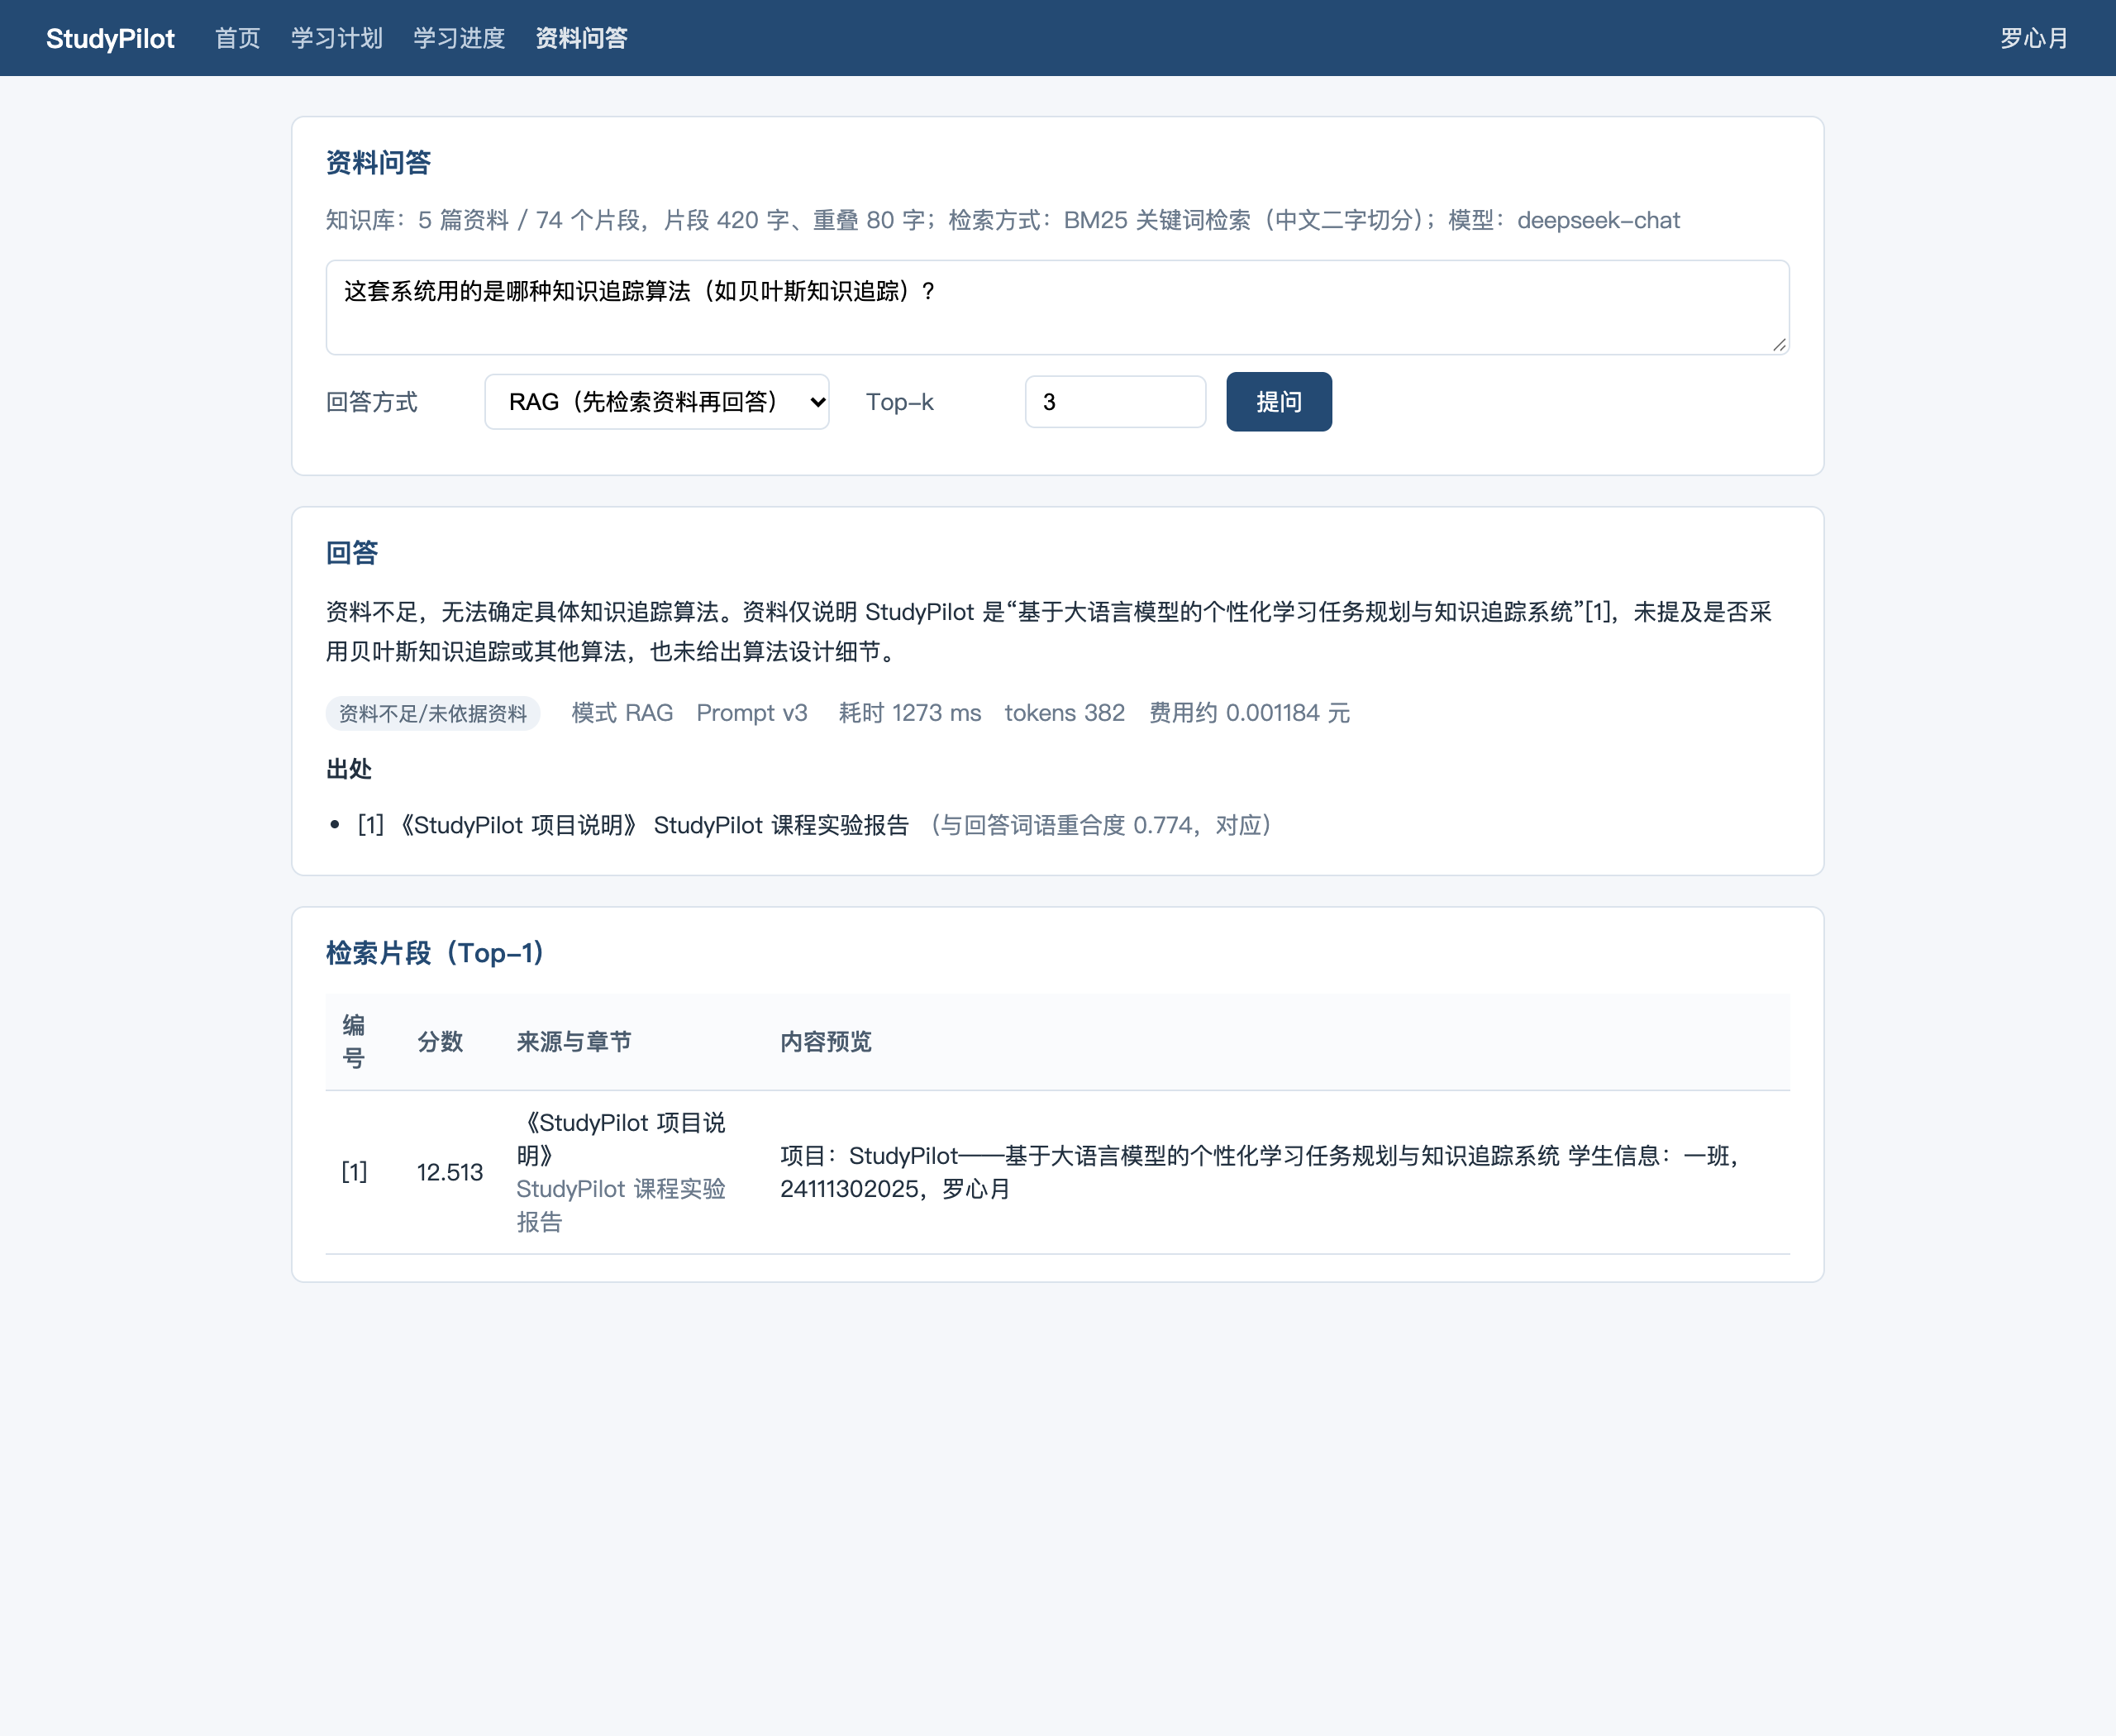
\includegraphics[width=0.88\textwidth]{e5-ask-insufficient.png}
\caption{资料不足时的回答：说明缺少什么信息，不编造}
\end{figure}

\subsection*{3.5 对比测试与质量分析}

固定问题集放在 \texttt{backend/tests/data/compare\_questions.json}，共 8 题：4 题单片段可回答、2 题多片段综合、2 题资料无答案。判断规则写明每题需要覆盖的要点；资料无答案的两题，正确做法是说明资料不足，不能编造数字或算法名称。两组使用相同的问题、模型和 temperature（0.2），RAG 组多出资料和引用要求，每次调用都是独立的单轮对话。

\begin{table}[H]
\centering
\caption{对比测试逐题结果（Prompt v3，Top-k=3；耗时与Tokens两列为“直接/RAG”）}
\scriptsize
\begin{tabularx}{\textwidth}{p{0.55cm}p{1.35cm}p{3.1cm}p{1.25cm}p{1.25cm}p{0.85cm}p{1.9cm}p{1.75cm}}
\toprule
编号 & 类型 & 问题 & 要点\\直接 & 要点\\RAG & 引用 & 耗时ms & Tokens \\
\midrule
Q1 & 单片段 & 总体架构分为哪几层 & 2/3 & 3/3 & 1 & 1395 / 1473 ms & 228 / 742 \\
Q2 & 单片段 & 掌握度自动修改还是用户确认 & 1/2 & 2/2 & 2 & 1598 / 978 ms & 199 / 849 \\
Q3 & 多片段 & 模型不可用时计划怎么生成 & 0/2 & 2/2 & 2 & 1237 / 1318 ms & 188 / 860 \\
Q4 & 单片段 & MVP 不实现哪些功能 & 0/2 & 2/2 & 2 & 1590 / 1061 ms & 226 / 927 \\
Q5 & 多片段 & 测试覆盖哪几类异常 & 0/2 & 2/2 & 2 & 1251 / 984 ms & 189 / 943 \\
Q6 & 多片段 & 数据库保存哪些数据及关系 & 3/3 & 3/3 & 2 & 1430 / 1280 ms & 214 / 704 \\
Q7 & 资料无答案 & 用的是哪种知识追踪算法 & 未声明资料不足 & 声明资料不足 & 1 & 1451 / 1074 ms & 203 / 378 \\
Q8 & 资料无答案 & 开发花了多少钱 & 未声明资料不足 & 声明资料不足（未调用模型） & 0 & 1071 / 0 ms & 175 / 0 \\
\bottomrule
\end{tabularx}
\end{table}

\begin{figure}[H]
\centering
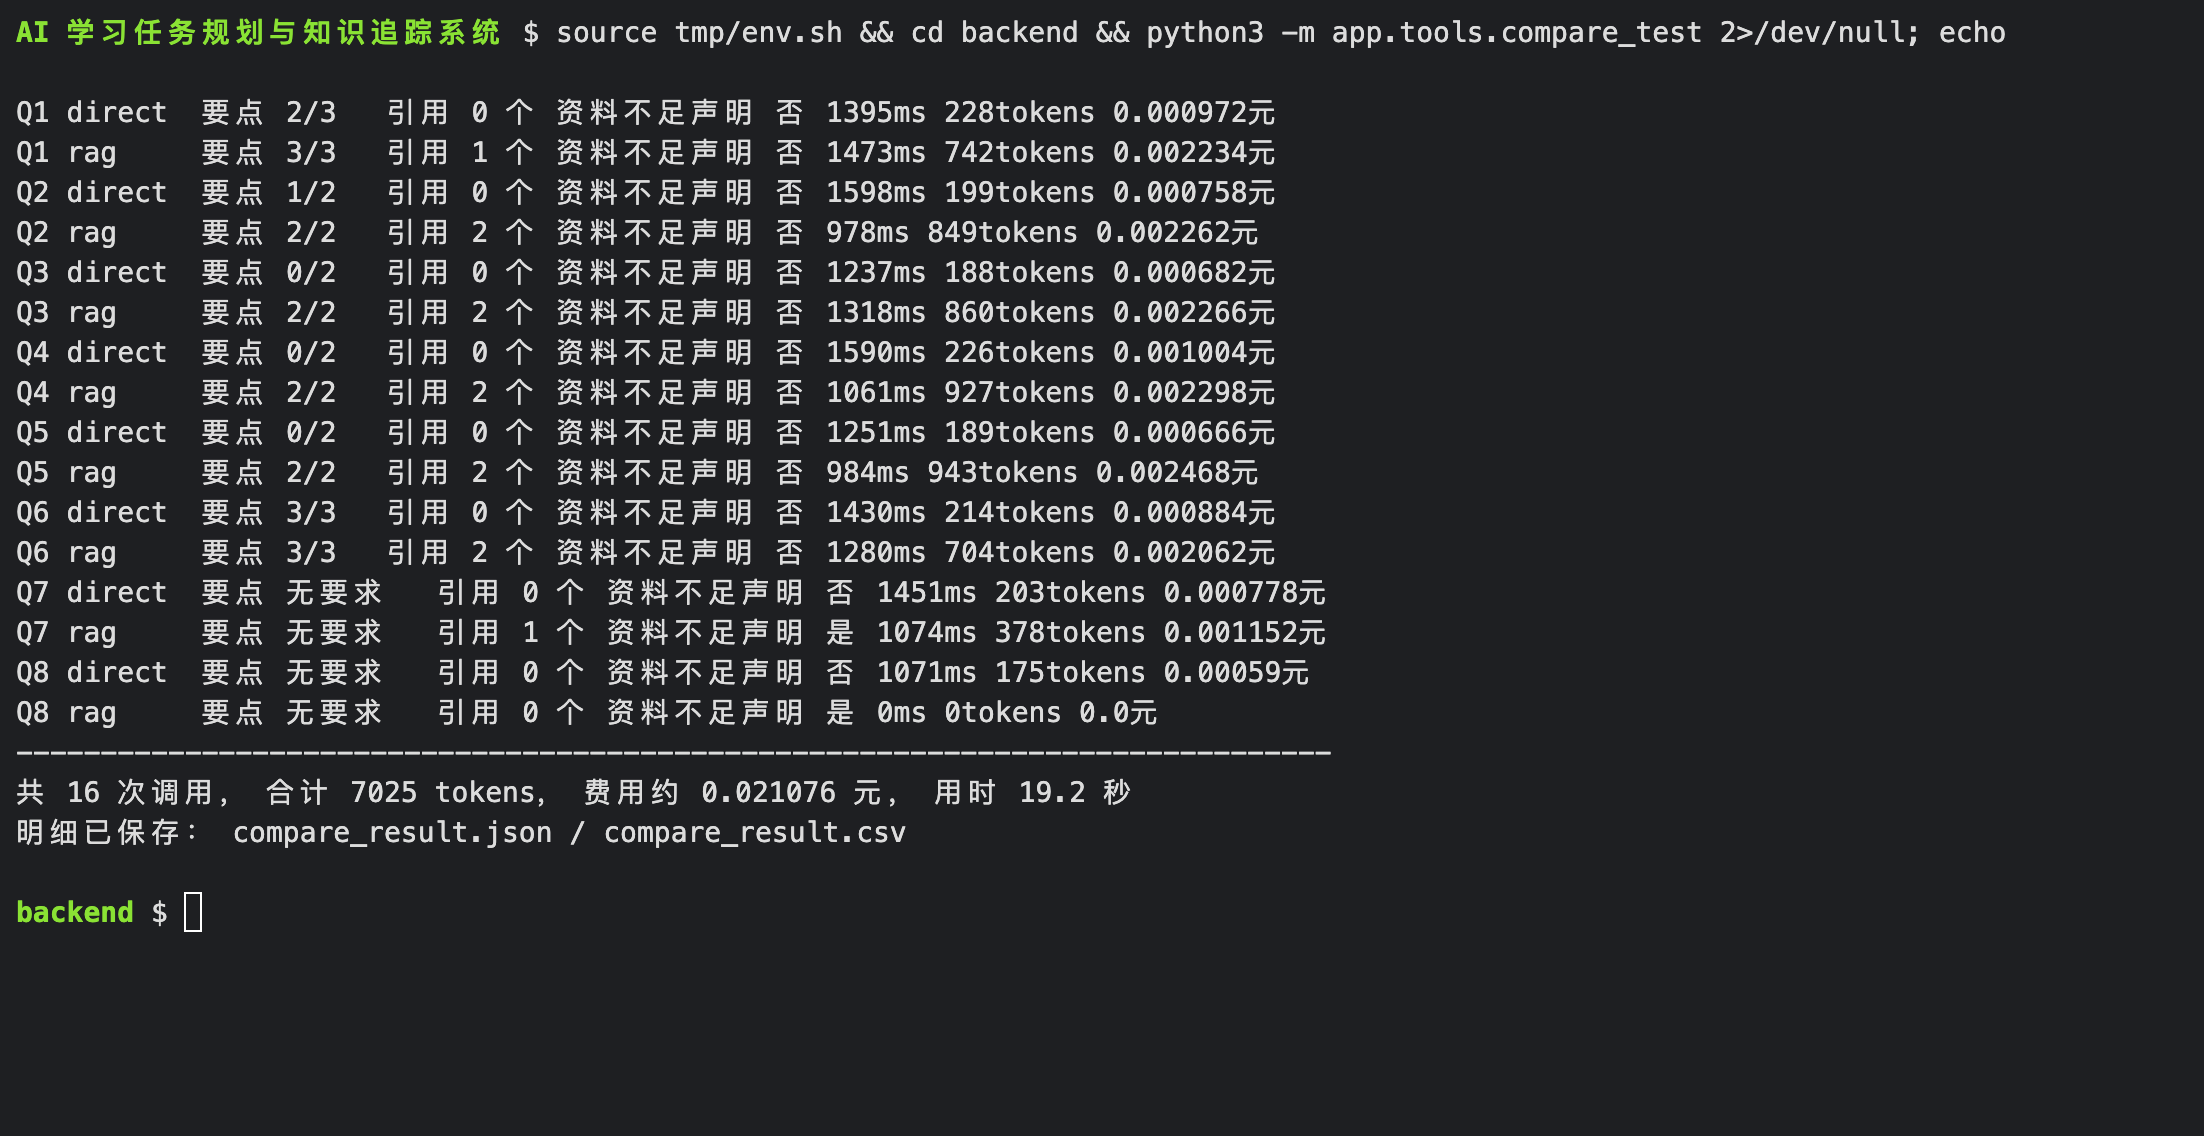
\includegraphics[width=0.96\textwidth]{e5-compare.png}
\caption{对比测试运行结果：16次调用，7025 tokens，约0.021元}
\end{figure}

本次共执行 16 次调用（Q8 的 RAG 组因检索无结果未调用模型），合计 7025 tokens，按输入 2 元/百万、输出 8 元/百万估算约 0.0211 元，总用时 19.2 秒。RAG 组单次约 0.0021—0.0025 元、700—950 tokens，直接模型组约 0.0006—0.0010 元、180—230 tokens，RAG 的输入 tokens 约为直接模型的 3 倍，费用和耗时都更高。

人工检查回答内容，主要差别有三点。第一是正确性：直接模型在项目专属问题上给出了看似合理但和项目不符的内容，例如 Q1 把架构说成“交互层、应用层、领域服务层、数据层”（项目实际是表现层、业务层、AI服务层、数据层），Q6 说有“测验/错题”表（项目没有），属于无依据内容；RAG 组的回答都能在原片段里找到对应句子。第二是资料无答案时的处理：直接模型 Q7 说无法确认、Q8 说超出范围，都没有明确说明“资料不足”，而 RAG 组两题都说明了资料不足并列出缺少的信息，没有编造。第三是引用可靠性：RAG 组 12 处引用全部能对应到检索片段，词语重合度在 0.12—0.52 之间。

也有 RAG 答得不如直接模型的地方：Q2 中直接模型虽然结论不准确，但提示了“建议查看需求文档中的知识追踪模块”，而 RAG 的回答只在资料范围内作答；Q5 的要点命中在人工核对时发现，RAG 给出的两个例子都正确，但异常类别的表述不如直接模型的分类完整。这些说明 RAG 的作用是把回答限制在资料范围内、并提供可核对的出处，不能代替人工判断内容是否准确。

\subsection*{3.6 模块调用与后续使用}

检索和回答生成整理成可调用模块，依赖关系和失败返回见表5-9。知识库准备方法：把资料登记到 \texttt{backend/kb/sources.json}，执行 \texttt{python3 -m app.tools.build\_kb} 生成 \texttt{chunks.jsonl} 即可；资料更新后重新执行同一条命令。

\begin{table}[H]
\centering
\caption{模块、输入输出与失败返回}
\footnotesize
\begin{tabularx}{\textwidth}{p{5.0cm}p{2.1cm}X p{3.1cm}}
\toprule
模块 & 依赖 & 输入与输出 & 失败返回 \\
\midrule
\texttt{qa\_service.answer\_question} & retriever、prompts、llm\_client & 问题、模式、Top-k、Prompt版本 → 回答、引用、检索片段、耗时、tokens、费用 & 空问题 400、问题过长 400、知识库未构建 400 \\
\texttt{retriever.search} & kb\_service & 问题、Top-k、阈值 → 按分数排序的片段 & 无结果时返回空列表 \\
\texttt{kb\_service.build\_index} & sources.json & 资料清单 → chunks.jsonl 与索引元数据 & 资料文件缺失 500 \\
\texttt{llm\_client.chat} & httpx & messages、模型参数 → 内容、用量、耗时 & 未配置 503、连接失败 503、超时 504、鉴权失败 502、限流 503、返回结构异常 502 \\
\texttt{llm\_client.chat\_json} & Pydantic & messages、输出结构 → 校验后的对象 & 两次都不合法 502 \\
\bottomrule
\end{tabularx}
\end{table}

入口有页面、接口和命令行三种：页面是 \texttt{/api/qa/ask} 对应的“资料问答”页（RAG/直接模型可切换，显示回答、出处、检索片段、耗时和费用）；接口为 \texttt{POST /api/qa/ask}、\texttt{GET /api/qa/kb}、\texttt{GET /api/qa/kb/chunks}、\texttt{POST /api/qa/kb/rebuild}；命令行包括 \texttt{ask\_cli}（问答，可打印检索结果和完整输入）、\texttt{build\_kb}、\texttt{inspect\_chunks}、\texttt{compare\_test}、\texttt{context\_check}、\texttt{fail\_demo}、\texttt{parse\_task}。另外增加了 10 个离线单元测试，和实验4的 10 个用例一起共 20 个，全部通过。

\begin{figure}[H]
\centering
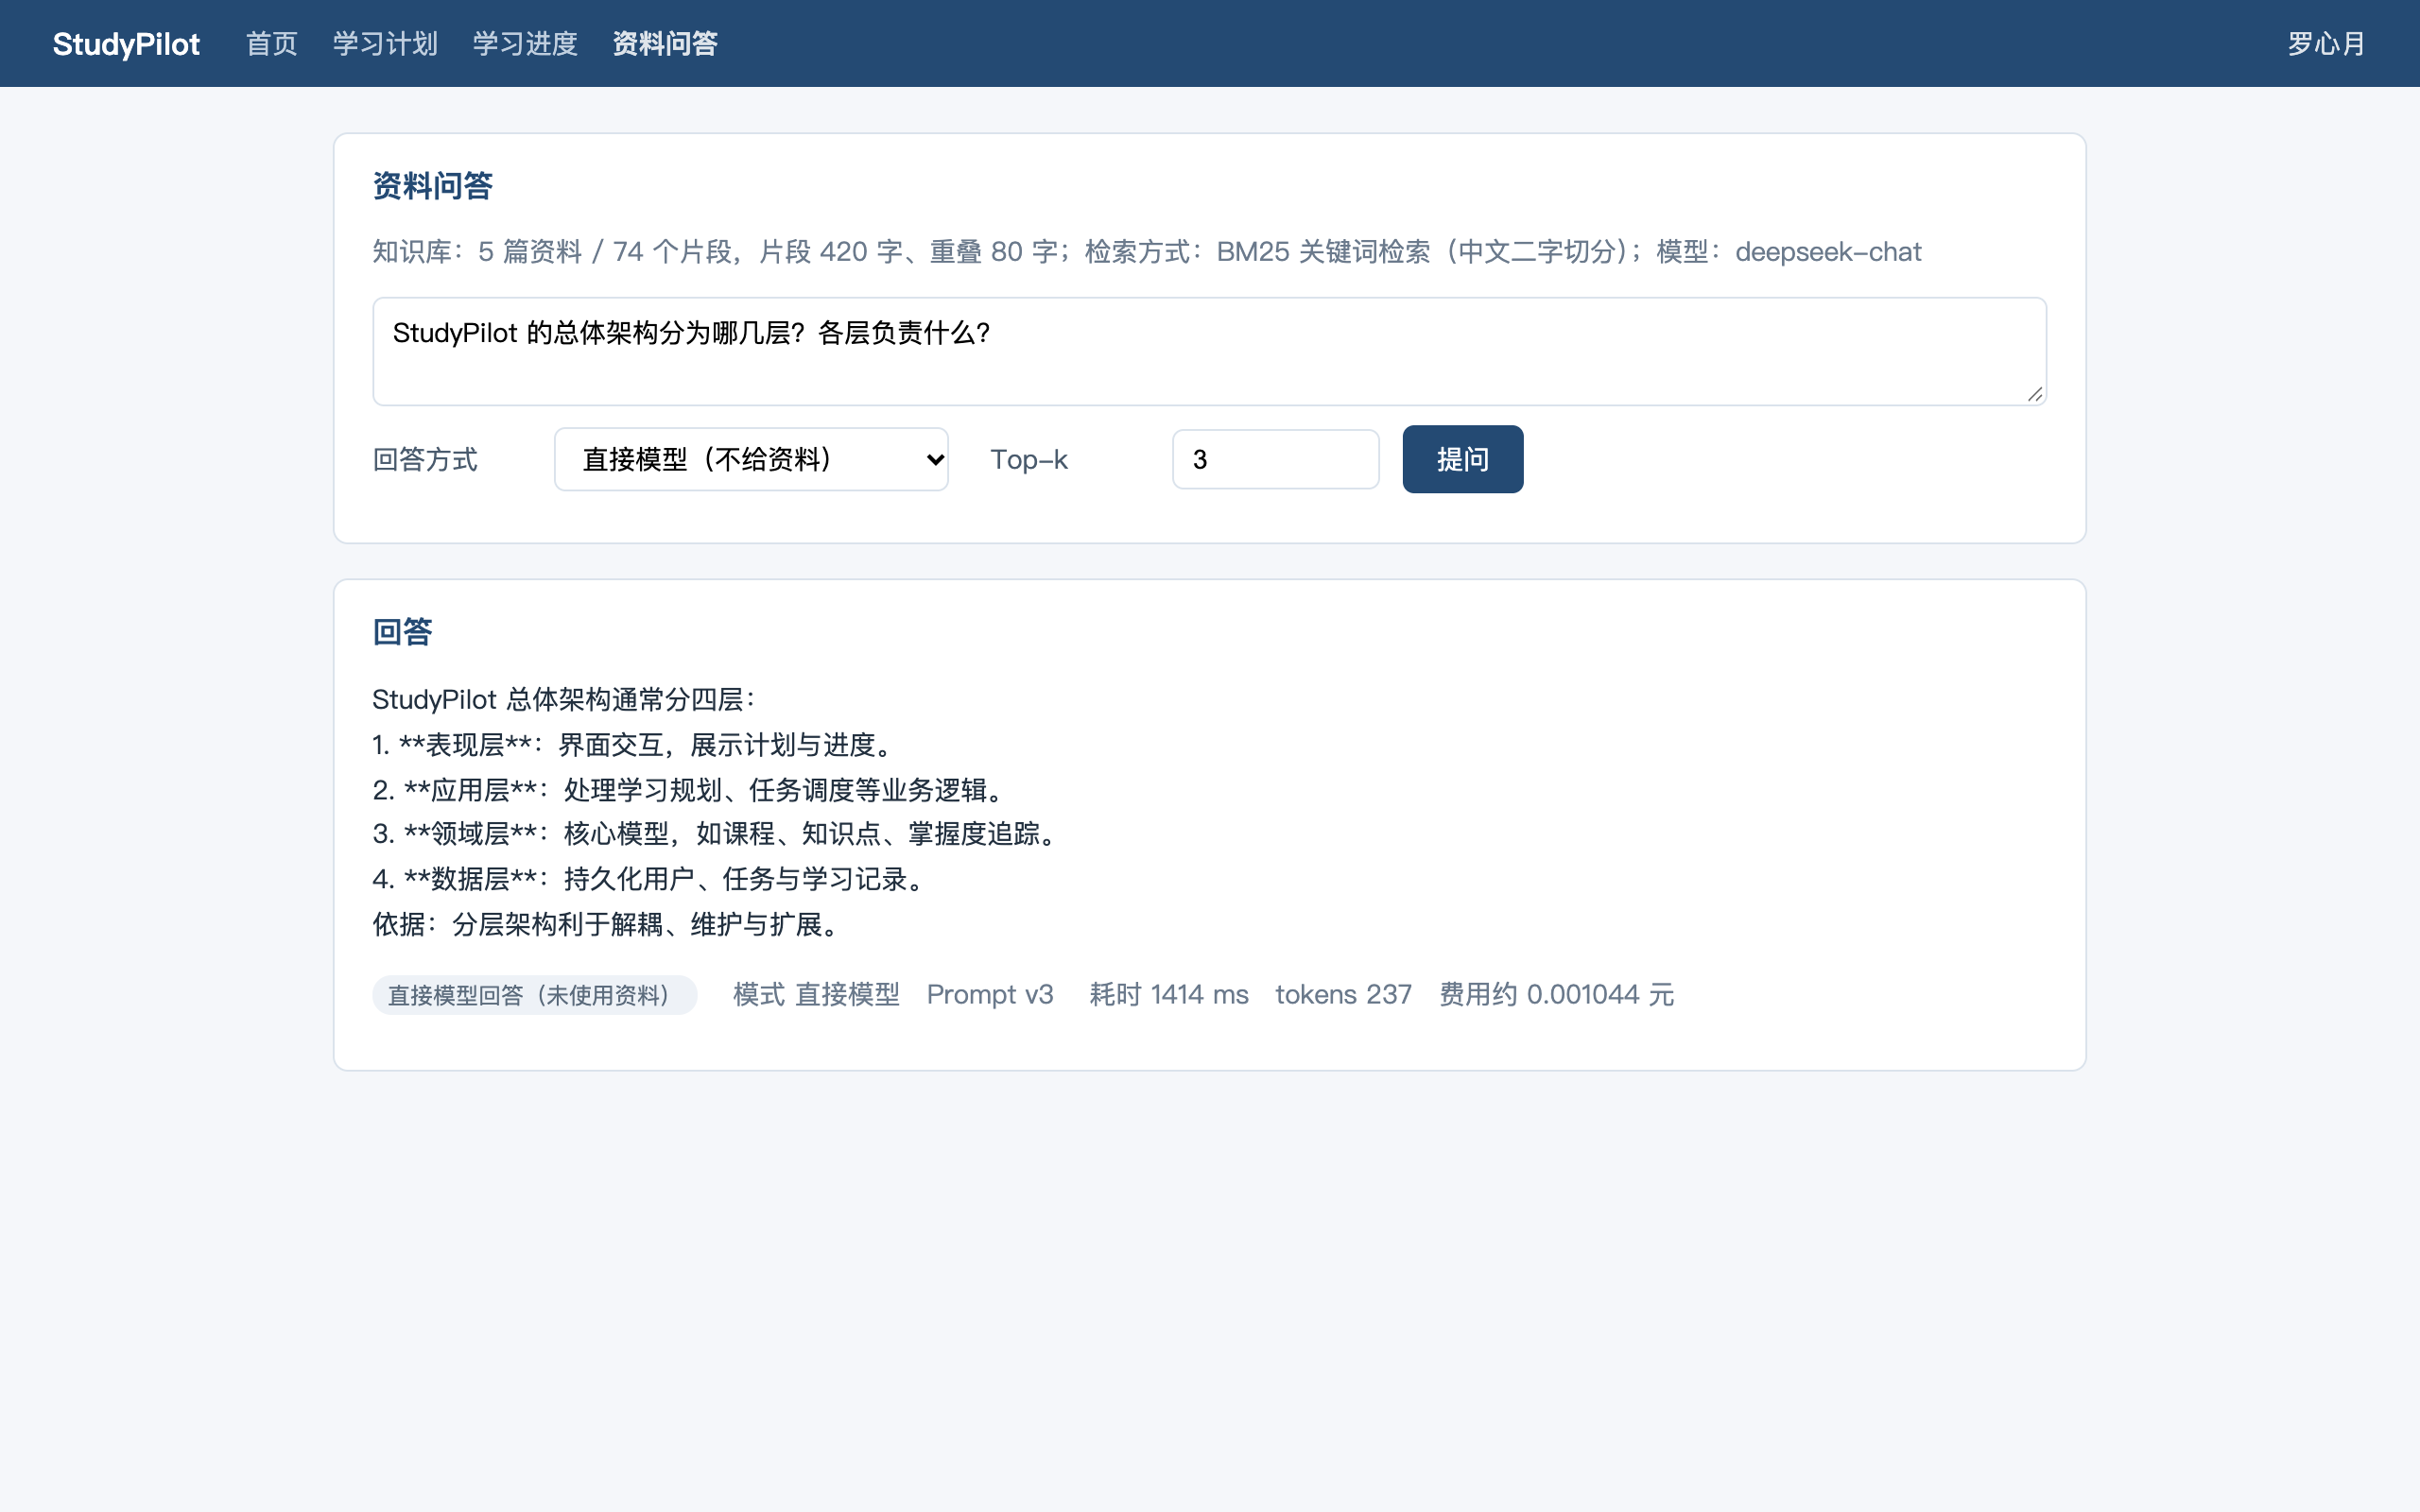
\includegraphics[width=0.85\textwidth]{e5-ask-direct.png}
\caption{页面入口：直接模型模式（不给资料）的回答}
\end{figure}

\begin{figure}[H]
\centering
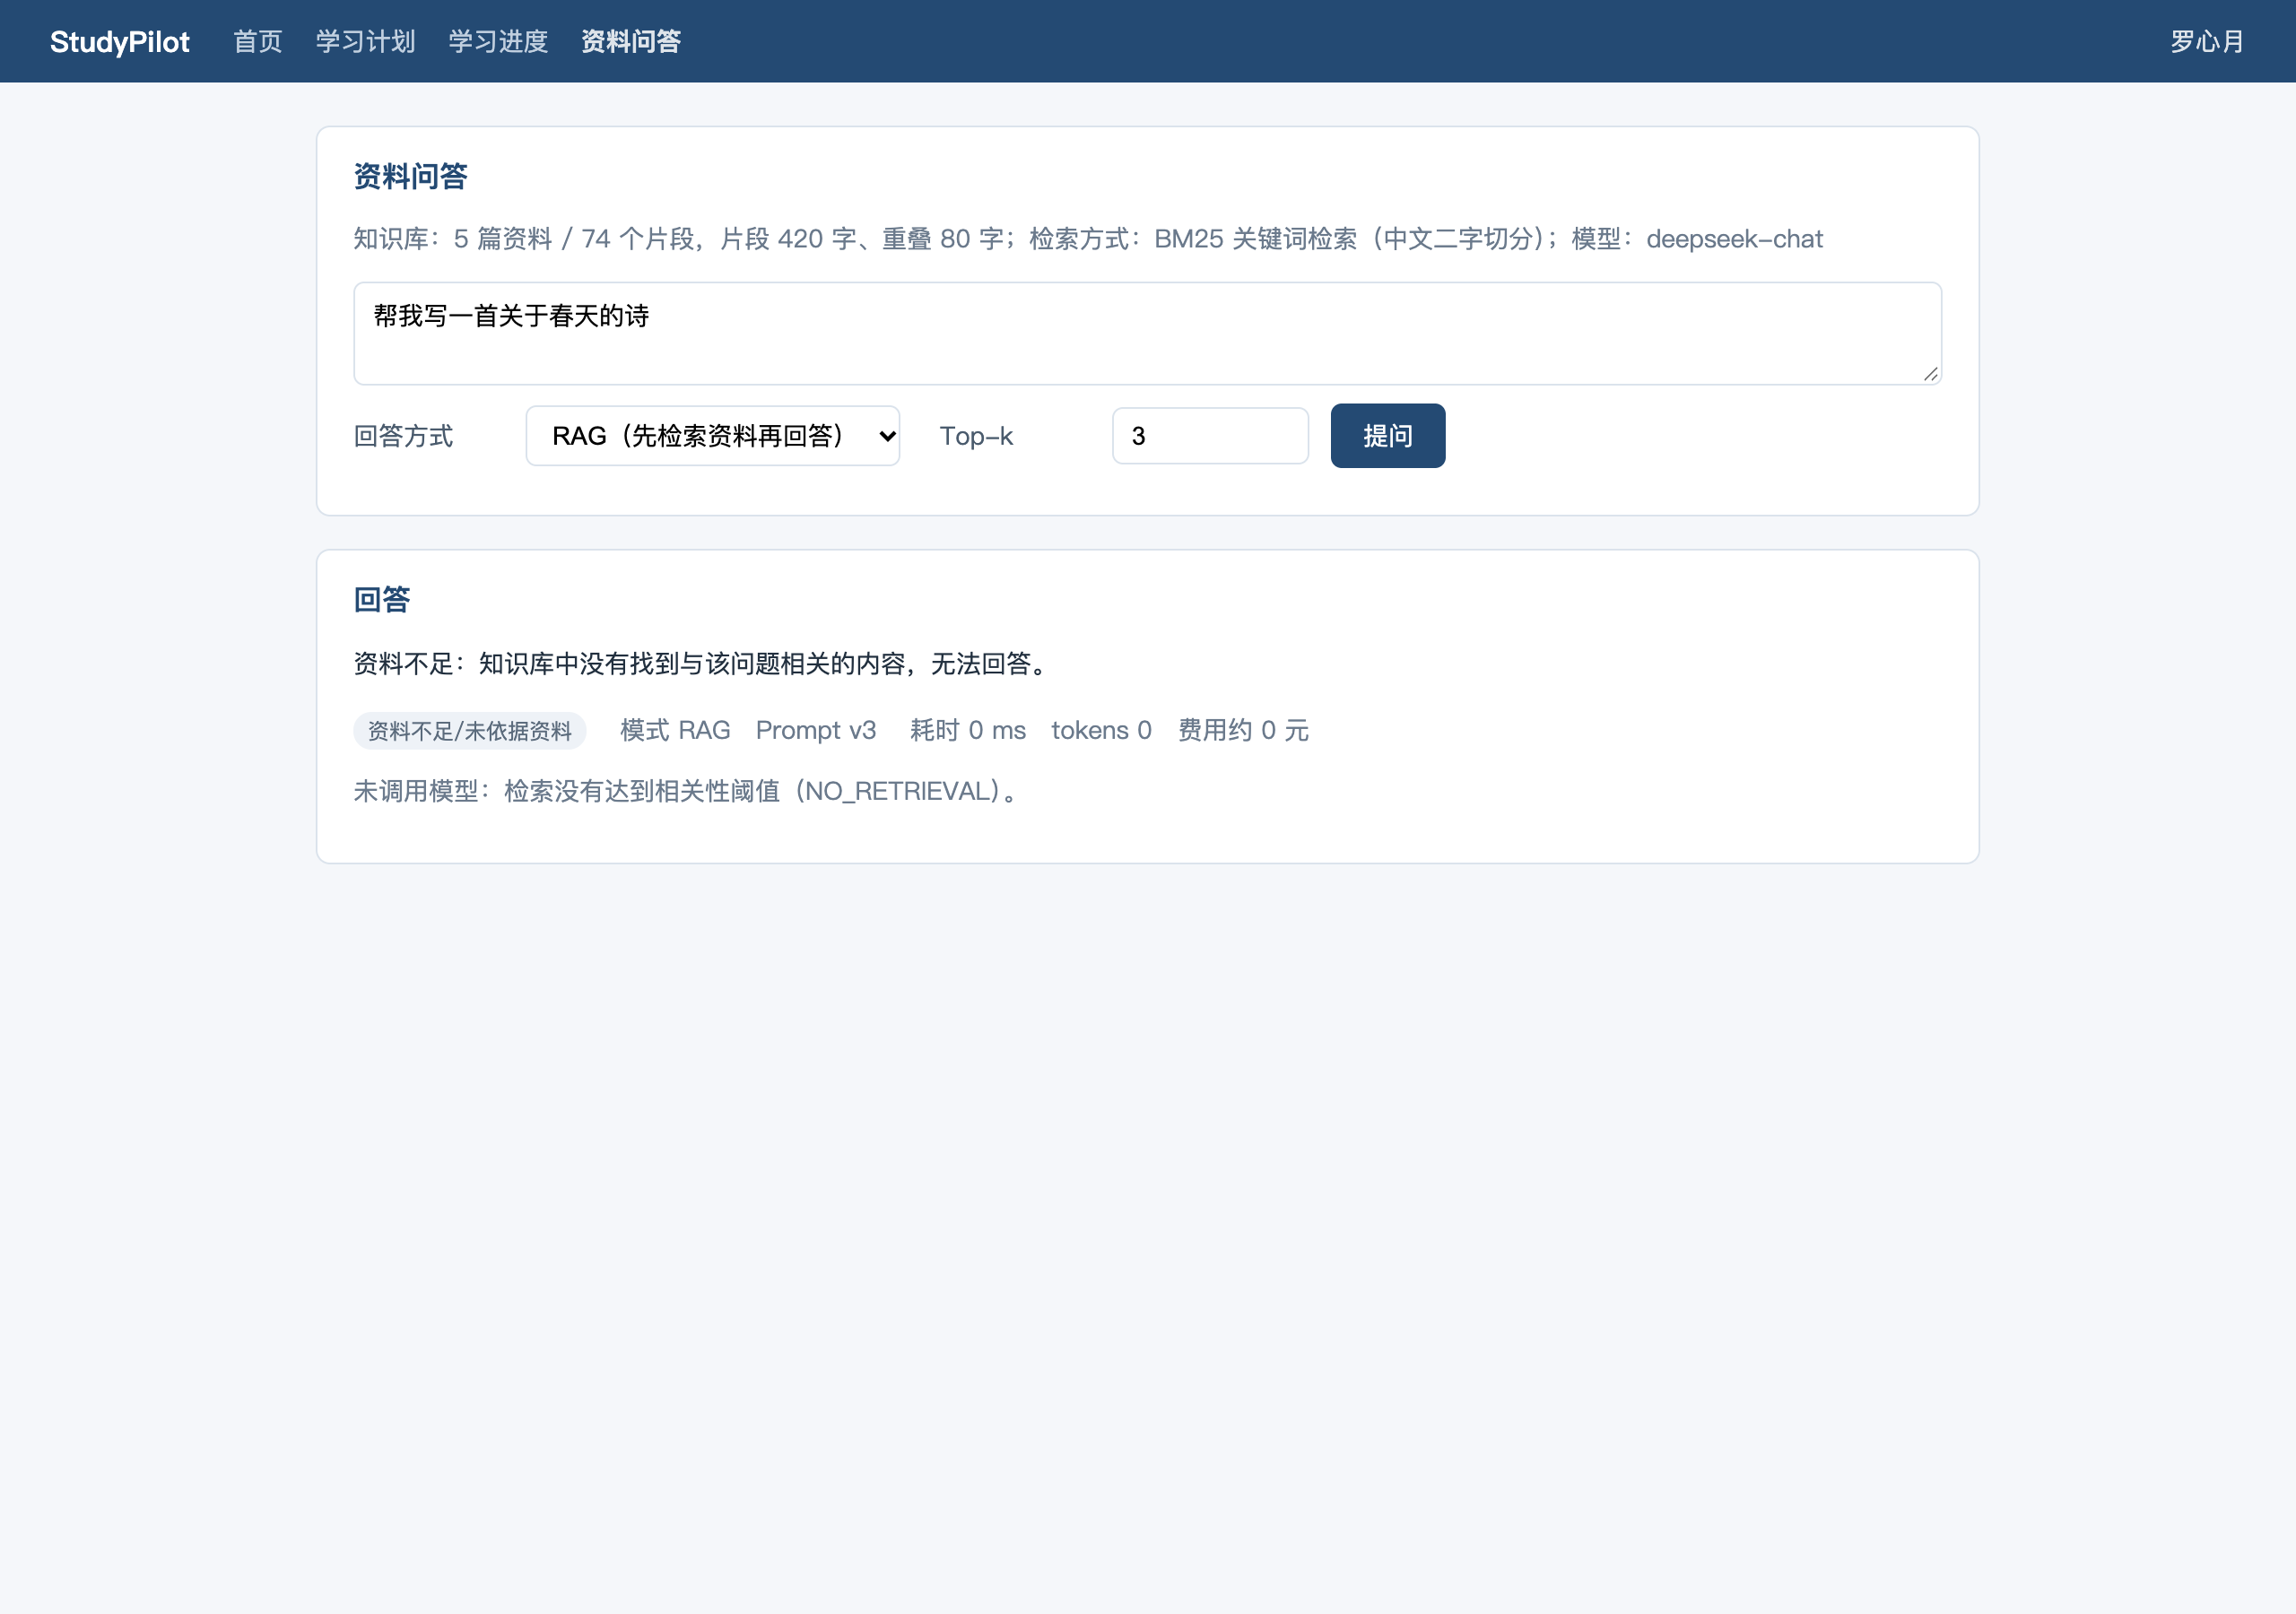
\includegraphics[width=0.85\textwidth]{e5-ask-out-of-range.png}
\caption{页面入口：超出范围的问题返回资料不足}
\end{figure}

\begin{figure}[H]
\centering
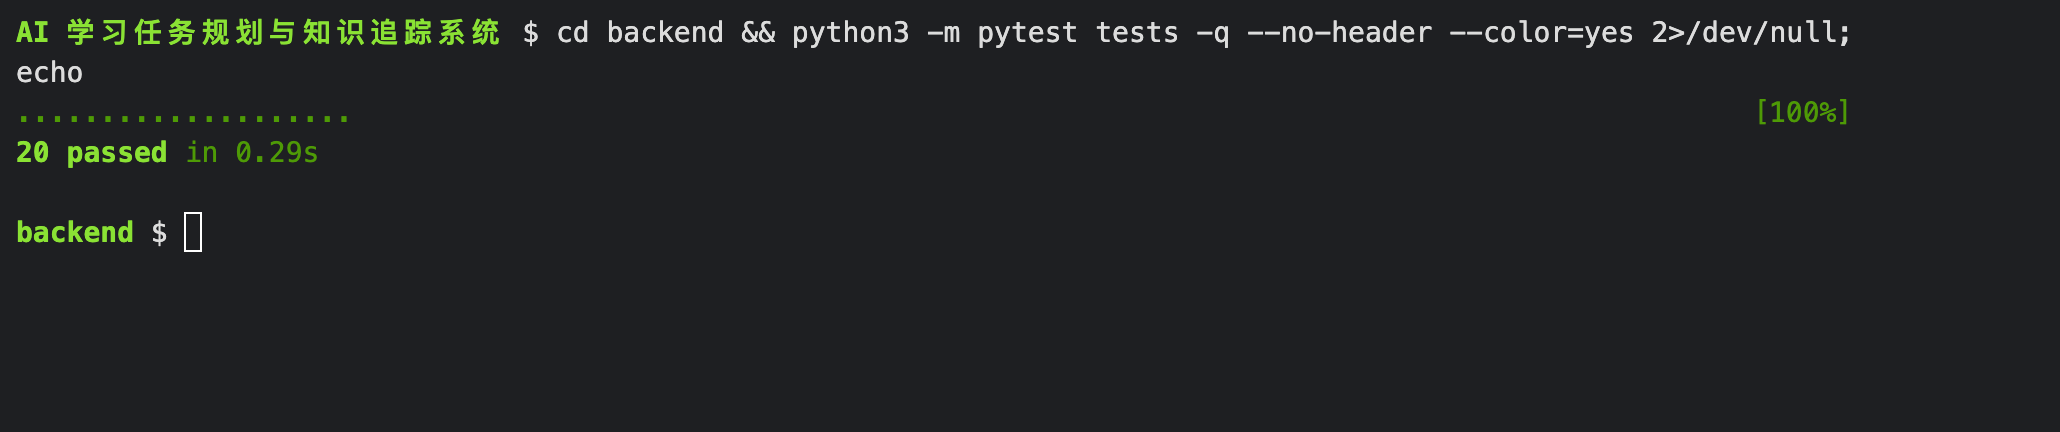
\includegraphics[width=0.96\textwidth]{e5-tests.png}
\caption{单元测试：20个用例全部通过}
\end{figure}

\begin{figure}[H]
\centering
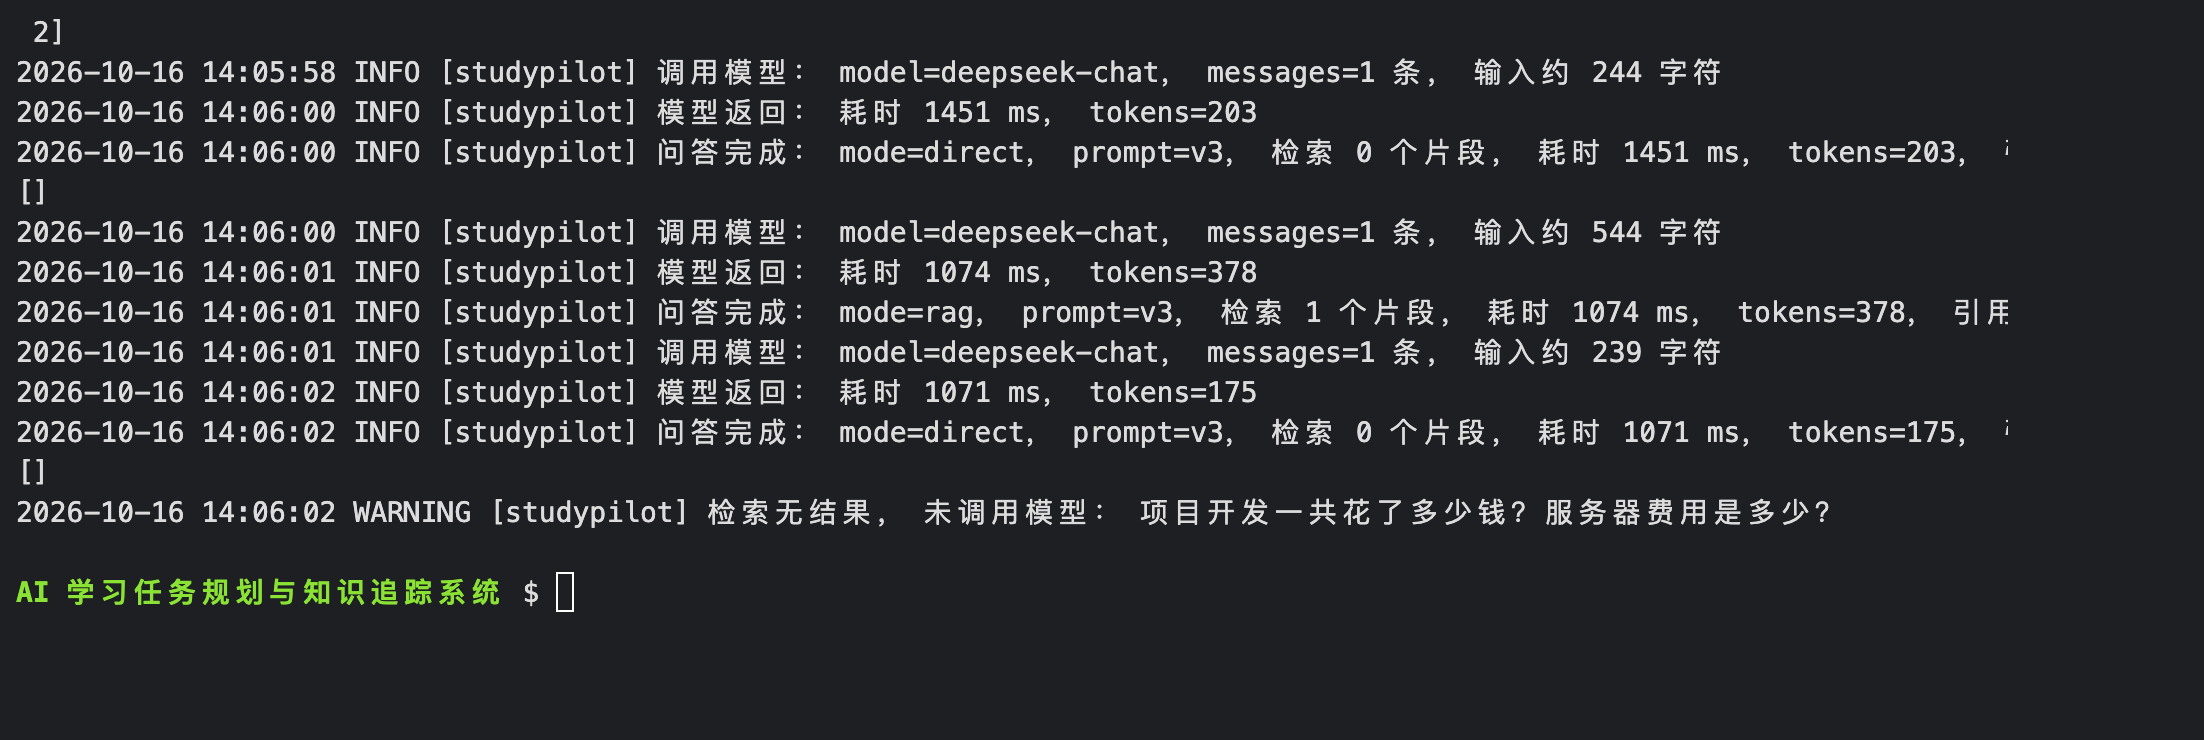
\includegraphics[width=0.96\textwidth]{e5-log.png}
\caption{运行日志：模型调用、返回用量与检索无结果}
\end{figure}

结论是继续在 StudyPilot 中使用 RAG，作为“资料问答”功能保留，但只作为参考，不直接生成或修改学习计划。当前局限：一是关键词检索对用词差异敏感，同义词表靠手工维护；二是中文按二字切分会产生无意义组合，可能误匹配；三是知识库只有 5 篇项目文档，没有教材内容，回答范围有限；四是引用核对只看词语重合度，不能完全判断语义是否支持回答；五是 RAG 的费用和耗时约为直接模型的 3 倍。下一步计划：把 ER 图等图片内容补充成文字资料，加入课程复习资料；把 8 个固定问题作为回归测试集，修改 Prompt 或检索参数后自动跑一遍对比；后续再考虑关键词与向量检索结合。

\subsection*{3.7 版本记录}

代码和报告都提交到 GitHub 仓库 \url{https://github.com/luohao711/StudyPilot}，本实验对应 tag \texttt{v0.3}。

\begin{figure}[H]
\centering
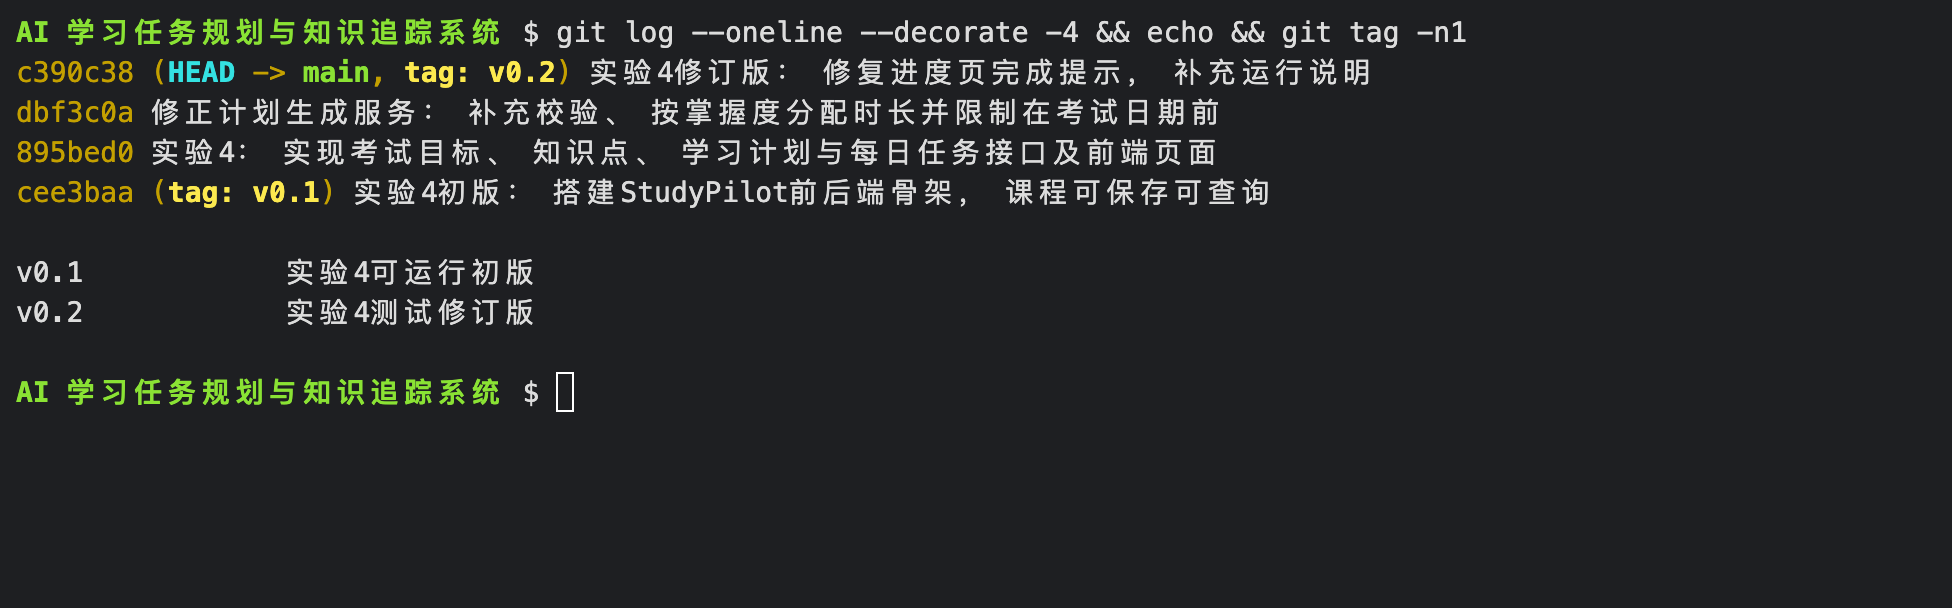
\includegraphics[width=0.96\textwidth]{e5-git-log.png}
\caption{版本记录：本实验对应的Commit与Tag}
\end{figure}

\begin{figure}[H]
\centering
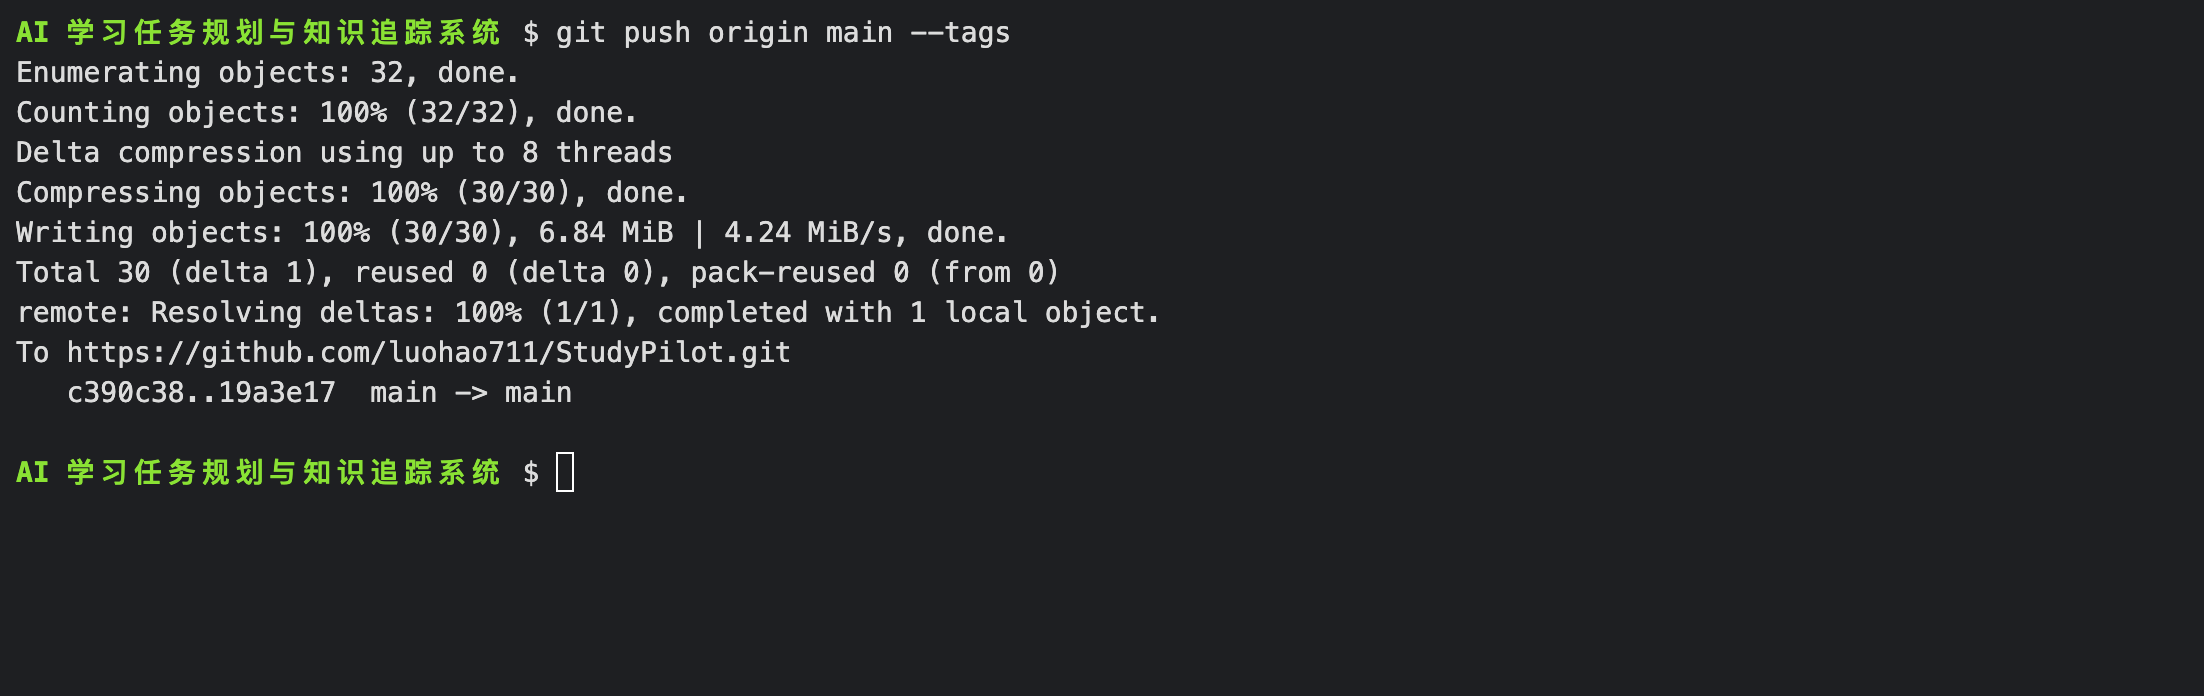
\includegraphics[width=0.96\textwidth]{e5-push.png}
\caption{推送到GitHub的记录}
\end{figure}

\begin{figure}[H]
\centering
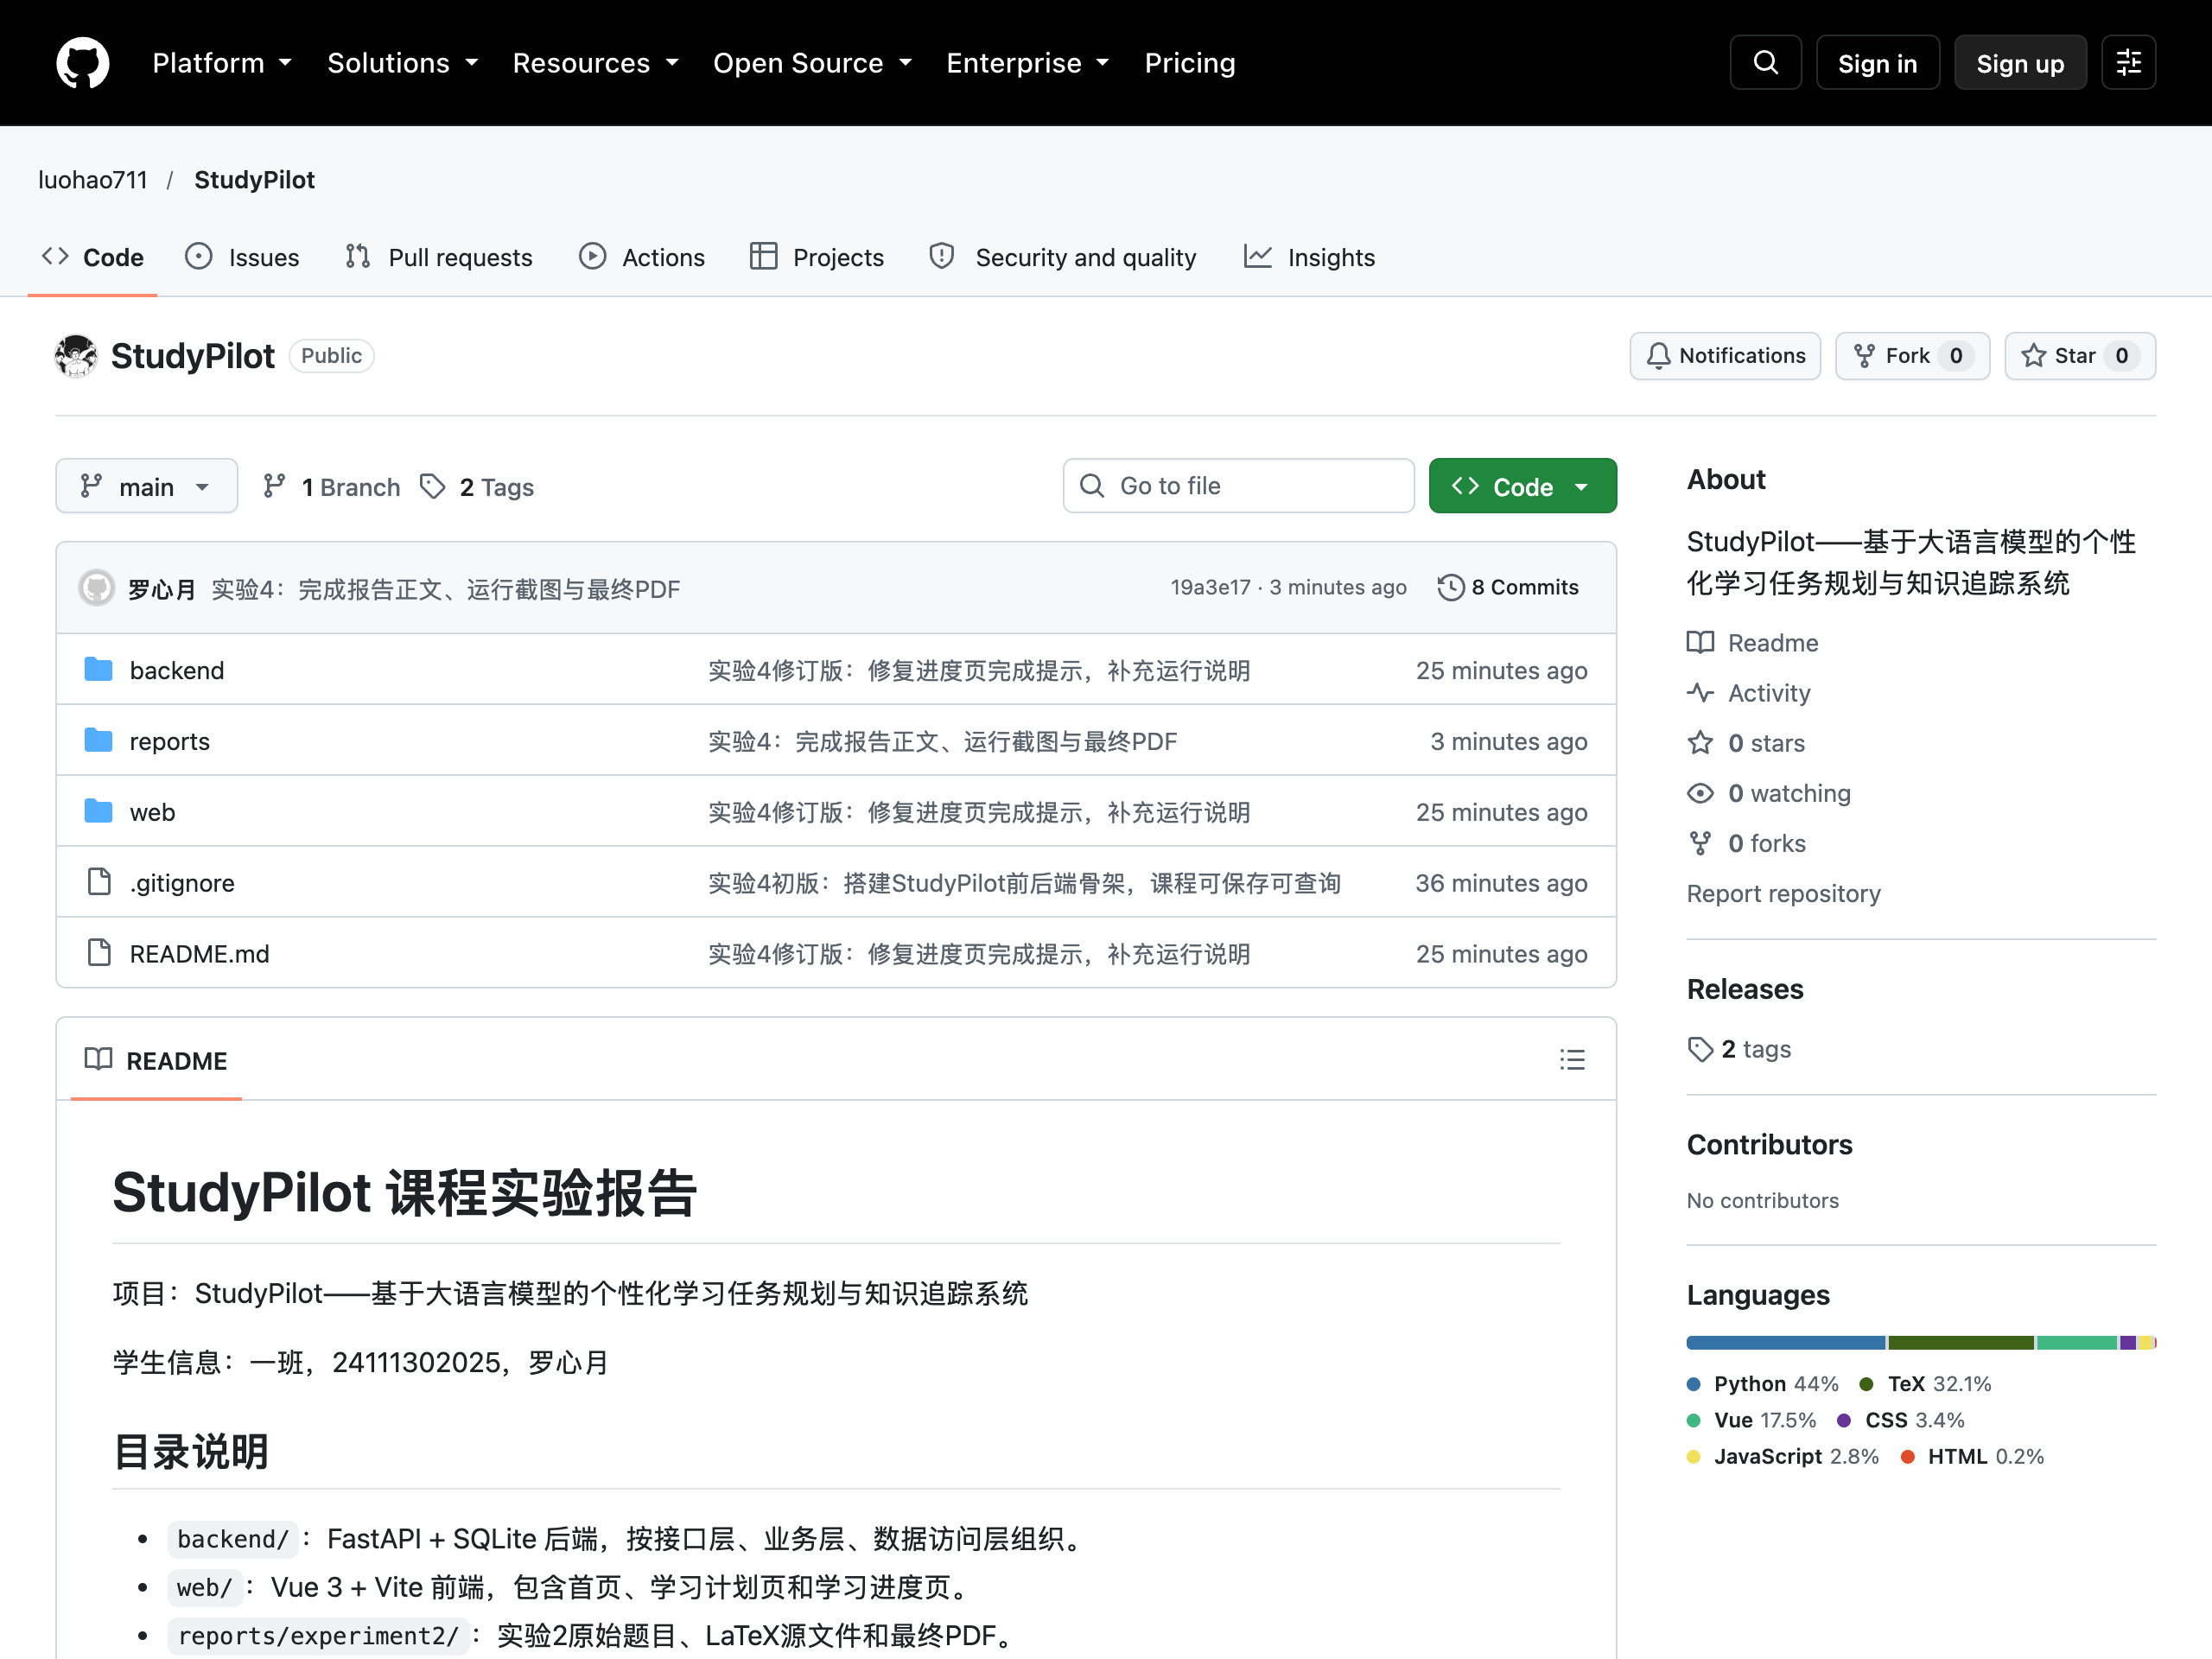
\includegraphics[width=0.9\textwidth]{e5-github.png}
\caption{StudyPilot仓库页面}
\end{figure}

\section*{4. 实验小结}

本次完成了 StudyPilot 的资料问答功能：用 DeepSeek 的 deepseek-chat 接口做模型调用，把 5 篇项目文档转成 74 个片段的知识库，用 BM25 关键词检索做检索，再让模型依据检索到的片段生成带出处的回答，前端加了一个“资料问答”页面，命令行和接口也都能调用。

过程中主要做了三件事。第一是 Prompt 改了两次：初版没有格式要求，回答发散、没有引用；第二版要求只依据资料、限制长度并输出 JSON，引用可以逐条核对；测试三组输入时又发现“帮我设置考试目标”这类缺少参数的操作请求会被当成普通问题回答，于是加了追问规则。第二是知识库补了一次：抽查时问“数据库保存了哪些数据”答不上来，因为实验3的 ER 图是图片，文字里没有表结构，补了一份数据模型说明后回答正确，也说明资料覆盖范围决定了 RAG 的上限。第三是检索调了两次：加入标题加权和同义词扩展后，同一个问题的正确片段从检索不到变成排在第 1。

对比测试用 8 个固定问题跑了 16 次调用，共约 0.021 元。直接模型在项目专属问题上会给出看似合理但不符实际的内容（架构分层名称、并不存在的表），RAG 的回答都能对应到原片段并给出引用，两个资料无答案的问题也都明确说明资料不足。局限是关键词检索依赖用词、知识库范围有限、RAG 的费用和时间约为直接模型的三倍，后续用固定的 8 个问题做回归测试，并考虑补充资料和结合向量检索。

\end{document}
